% Kapitel - Methodology
\section{Methodology}

The literature review revealed a significant opportunity to enhance the passenger experience in future autonomous vehicles. While interactive e-textiles and \gls{WSD}s present a promising alternative to current \gls{HMI} paradigms, there is a lack of established design guidelines for creating intuitive, "walk-up-and-use" interactions for novice users. Specifically, a research gap exists in understanding how different levels of feedforward can guide users to interact with such novel interfaces effectively and enjoyably.

\subsection{Research Approach}

To address this gap in a user-oriented manner, this thesis employs the Human-Centered Design, or \gls{HCD} \cite{noauthor_din-9241-110_nodate, norman_design_2013} process. The methodological framework is built upon an adaptation of the well-established Double-Diamond design model \cite{norman_design_2013}. This model advocates for a process of first diverging to explore a problem space widely before converging on a specific problem, and then repeating this pattern to develop and refine a solution.
Given the multi-stage nature of this research, spanning from foundational research and prototyping to iterative user testing and final evaluation, the traditional Double-Diamond has been expanded into a "Quad-Diamond" process. This adapted model, visualized in Fig. \ref{fig:diamond}, more accurately reflects the extensive and iterative journey undertaken.

\begin{figure} [h!]
    \centering
    \includegraphics[width=1\linewidth]{images/Quad Diamond.png}
    \caption{Illustration of this work's Quad Diamond research approach. Adapted from Norman \cite{norman_design_2013}.}
    \label{fig:diamond}
\end{figure}

The four key phases of this approach are:

\begin{enumerate}
    \item \textbf{Foundational Research and Problem Definition:} The first diamond focuses on understanding the fundamental issues through an extensive literature review to discover user needs in \gls{AV}s and define the specific research problem. This process can be found in Chapter \ref{sec:RelatedWork}.
    \item \textbf{Conceptual Design and Initial Prototyping:} The second diamond moves into the solution space, involving the design exploration of interaction concepts and feedforward strategies and converging them into an initial, testable prototype (Version 1).
    \item \textbf{Pre-Study and Prototype Refinement:} The third diamond represents a critical iterative cycle with a formative role \cite{kendrick_formative_2019}. A qualitative pre-study was conducted to gather broad qualitative feedback on the initial prototype, which was then analyzed to implement on a refined and improved design (Version 2).
    \item \textbf{Final Evaluation and Guideline Formulation:} The final diamond involves a comprehensive, summative user study aiming to evaluate various feedforward levels though testing of the refined prototype and gather extensive quantitative and qualitative data \cite{kendrick_formative_2019}. This data is then synthesized to converge on the final output: a set of empirically-grounded design recommendations.
\end{enumerate}

Throughout these four phases, the core principles of the \gls{HCD} process; observation, idea generation, prototyping, and testing \cite{norman_design_2013}, are applied iteratively. This ensures that the user remains at the center of the development process, and that the final design guidelines are directly informed by their needs, behaviors, and experiences.

\subsection{Conceptual Design and Initial Prototyping (Version 1)}
\begin{comment}
Okay Next I want to go into the Conceptual Design and Initial Prototyping. I have a few things I want to explain there. I will just dump it here in a super short form here to each point and aspect I mention there is a lot of details to report. I'd love if you can help me organize it for a good and logical flow into something like a skeleton.

Alright so I gathered non-driving related in-vehicle interactions that are common today plus a few that are exclusively interesting for AVs or the technologies of my HMI paradigm. 
I then explored various interaction metaphors for these use cases and defined elements for the textile interface and possible visualization concepts for the WSD, for each use case. I tried to keep in mind that these interaction are playful and fun to generate positive experiences.
I then tried to find common interactions and elements between the use cases or adapted some interactions to share common elements and from that build possible layouts of interactive elements that still support all possible interactions, while already considering the shapes shifting which allowed elements to also be hidden away and therefore allow for different interactions. That led me to find a layout of interaction elements that holistically works for the whole system (while still keeping in mind things like ergonomics and avoidance of false input and so on. 
I then defined the general size of the armrest and how much space the interactive elements take place on that surface and how exactly they are positioned. For that sketches in real size have been made. In the same step I started ideating the physical inherent feedforward cues by either leveraging shape shifting / deformability of the textile to make the building of the prototype feasible and adjust the layouts and positions slightly if necessary for ergonomics or feasibility. Furthermore a fabric was chosen to support the shape shifting e.g. through stretchy properties as well as fabric to leverage affordances itself. All design decisions have been made based on literature findings. The hardware has been carefully chosen and the prototyping software Blokdots made it controllable. 
I then analyzed the most diverse interactions and metaphors in the set of interactions I created and that way picked a set of non-driving related in-vehicle interactions and applications/use-cases to fully implement to the prototype to later evaluate in the user studies. I created a story line of different scenarios and interactions that will help future participants to vividly experience the prototype. 
After that I started designing the GUI for the WSD. I applied various design guidelines (mainly for usability) and I laid a lot of focus on the layout of elements as well as animations to support the interactions on the textile surface that act as inherent feedforward, so clarifying how to interact. Designed in Figma and made interactive in ProtoPie. I made sure to develop the prototype as nonlinear as possible so users at leas get the illusion that they have the freedom to move anywhere as if they are using a complete system. 
I then started to design and implement the augmented feedforward cues of light. The aim was to integrate them as seamlessly as possible, so the light projections followed the physical shapes of the interface perfectly. Moreover the projections have been blurred to integrate even more seamlessly into the surface as well as smooth animations emphasizing how to use the elements. The animations as well as colors have also been used to leverage the indication of functionality e.g. color of multiple choice option represented from the WSD or red as aborting. 
Then I started to design and implement the augmented feedforward cue of explicit text hints/instructions within the GUI. The aim was to show the functionality (and how to interact) by making the cues as unambiguous as possible while being short and concise. Some situation however required multiple text cues to be shown, therefore they have ether been displayed side by side or in intervals. 
The armrest has then been placed on height adjustable legs to ensure the perfect height for each participant. Feedback had only been implemented visually at that point, but was planned to be added on more modalities.

Where do I explain which feedforward levels I chose to explore and why????????????

Also somewhere I have to walk through all scenarios in detail and explain all the interaction possibilities and how they look in various feedforward levels, but maybe I can do that for the final iteration? Nah it should be for bot versions, right?
\end{comment}
This section details the design process for the first iteration of the interactive textile and \gls{WSD} prototype. Following the divergent and convergent phases of the design diamond, the process began with a broad exploration of potential interactions and culminated in a functional prototype ready for preliminary testing.

\subsubsection{Defining Use Cases and Interaction Metaphors}

\paragraph{Identifying Potential Interactions:} \mbox{} \\
% The process started by gathering a comprehensive set of NDRAs to be performed within the in-vehicle user interface (so this excludes activities like working on a laptop or eating that don't require or can't be supported by the in-vehicle system and therefore don't require interaction with the system)
% This included common in-vehicle tasks from today's In-Vehicle Information Systems (IVIS) (e.g., media control, calls) and novel interactions suited for the AV context and the proposed HMI paradigm (e.g., interacting with points of interest displayed on the WSD). For each of these in-vehicle tasks all possible interactions within that task have been written down to later explore possible interactions concepts for each of them and considering they all have to be available withing the same applications/tasks. So for the music media control example task possible interactions that need to be suported are: play, pause, rewind, fastsforward, skip a song, go back a song and adjust volume and so on. 
The initial step in the conceptual design phase was a divergent exploration to identify a comprehensive set of potential user interactions with the \gls{AV} system. The process began by gathering a broad range of \gls{NDRA}s that would be performed using the in-vehicle \gls{HMI}. This scope intentionally excluded activities that do not require direct system interaction although they might be possible \gls{NDRA}s for \gls{HAD}, such as working on a personal laptop or eating, to focus on functions the proposed system needed to support.

The gathered activities included both \textbf{common tasks} found in contemporary in-vehicle infotainment systems, such as making calls, adjusting climate settings, and controlling media, as well as \textbf{novel interactions} uniquely suited to the \gls{AV} context and the proposed \gls{HMI} paradigm. These novel interactions have been ideated to support potentially popular \gls{NDRA}s identified in the literature \cite{berger_designing_2021, ahram_non-driving_2020, ahram_what_2020, pfleging_investigating_2016, stampf_deriving_2024, wilson_non-driving_2022}. For example, engaging with dynamic points of interest on the \gls{WSD}, which augments the real-world view, directly supporting the activity of looking out the window and observing the environment \cite{ahram_what_2020, pfleging_investigating_2016} and enabling shared interaction and social conversation with the vehicle passengers \cite{berger_designing_2021,  pfleging_investigating_2016, wilson_non-driving_2022}. Another example is an ambient soundscape mixer, allowing passengers to blend different sounds on a two-dimensional matrix to create an atmosphere suited for relaxation or focused work \cite{ahram_non-driving_2020, pfleging_investigating_2016, wilson_non-driving_2022}.

For each high-level application, a detailed breakdown of all necessary sub-interactions was created (see Table \ref{tab:ndra_interactions}) to ensure the final design would be robust and holistic. For instance, the "media control" task was broken down into essential functions that the interface must support: play, pause, skip forward, skip back, fast-forward, rewind, and volume adjustment. 
% This systematic collection of tasks and sub-interactions (see Table \ref{tab:ndra_interactions}) formed the foundational requirements for the subsequent design of the interaction metaphors and interface layout.

\begin{table}[h!]
\centering
\caption{Representative Sample of Identified Non-Driving Related Activities and Interactions}
\label{tab:ndra_interactions}
\begin{tabular}{|l|l|l|}
\hline
\textbf{High-Level Task / Application} & \textbf{Required Sub-Interactions} & \textbf{Interaction Type} \\ \hline
\textbf{Media Control} & Play / Pause & Toggle \\ \cline{2-3} 
 & Skip Forward / Back & Directional Action \\ \cline{2-3} 
 & Volume Adjustment & Continuous Input \\ \cline{2-3} 
 & Fast-Forward / Rewind & Continuous Input\\ \hline
\textbf{Phone Call} & Accept / Decline Call & Binary Choice \\ \cline{2-3} 
 & End Call & Single Action \\ \cline{2-3} 
 & Mute Microphone & Toggle \\ \hline
\textbf{Climate Control} & Adjust Temperature & Continuous Input \\ \cline{2-3} 
 & Adjust Fan Speed & Continuous Input \\ \cline{2-3} 
 & Select Airflow Zone & Selection \\ \hline
\textbf{Points of Interest} & Select a \gls{POI} & Pointing Action \\ \cline{2-3} 
 & Get More Information & Single Action \\ \cline{2-3} 
 & Zoom In / Out & Continuous Input \\ \hline
\end{tabular}
\end{table}

In addition to these application-specific functions, this exploratory phase also identified the need for universal, system-level interactions. To ensure predictable and intuitive navigation, it was determined that the \gls{HMI} must support a consistent method for a "back" gesture, a way to return to a "home" or main menu, a standardized approach for navigating menus and sub-menus, and a universal "select" or "confirm" action. These foundational interactions were deemed essential for creating a cohesive user experience across the entire system.

This systematic collection of tasks and sub-interactions formed the foundational requirements for the subsequent design of the interaction metaphors and interface layout.


\paragraph{Exploring Interaction Concepts:} \mbox{} \\
% With a set of required interactions established, the next divergent phase involved exploring various interaction metaphors for each use case. 
With a set of required interactions established, the next divergent phase involved exploring various \textbf{user interface metaphors} \cite{carroll_chapter_1988}. This is a common design approach that grounds \gls{UI} actions in a familiar framework, allowing users to transfer knowledge from a known source domain (e.g., tangible objects) to an unfamiliar target domain (the novel textile interface), which helps establish expectations and aids learnability \cite{carroll_chapter_1988, neale_chapter_1997}.  
Following the possibility-driven design framework \cite{desmet_towards_2012}, a key driver for this exploration was the goal of creating \textbf{positive, playful, and engaging experiences}. This approach was chosen to directly support the hedonic qualities that the literature identifies as crucial for the successful adoption of both autonomous vehicles \cite{detjen_how_2021} and e-textile technologies \cite{brauner_interactive_2017}.

The design focused primarily on "surface gestures", which Mlakar et al. \cite[pp.~1159]{mlakar_exploring_2021} define as "a class of gestures that are similar to touch gestures for touchscreens like touching the textile with one or multiple fingers or sliding them on the textile’s surface in a coordinated way". Following the key principles for intuitive design by Mortensen \cite{mortensen_how_nodate}, this decision was deliberately made to leverage user's prior experience with related products.
% With the ubiquity of touchscreens in technical devices, like in cars, a large spectrum of the population possess extensive familiarity with touchscreen interactions, which provides a strong foundation for intuitive use.
Given the ubiquity of touchscreens in modern consumer electronics and specifically within automotive infotainment systems, a broad user base possesses extensive familiarity with surface-based gestures, which provides a strong foundation for intuitive interaction. 

However, to avoid simply replicating digital controls on a new material, which is a potential pitfall noted by Gowrishankar et al. \cite{gowrishankar_strategy_2017}, a balanced approach was taken. 
% This hybrid strategy combined the familiarity of surface gestures with interactions that are unique to the textile medium. The unique affordances of the fabric, such as its deformable and shape-shifting qualities, were leveraged to enhance these familiar gestures, creating a novel yet understandable experience. 
This hybrid approach sought to augment, rather than simply copy, familiar interactions by leveraging the unique physical properties of textiles. Instead of occurring on a flat \gls{2D} plane like a touchscreen, gestures were designed for a 2.5D surface \cite{olwal_e-textile_2020}, where physical textures, profiles, and variations in material could guide the user's hand and enrich the tactile experience. 
%This method aimed to create interactions that felt intuitive due to their familiarity, yet novel and more engaging due to their physicality. 
% However, this exploration was not limited to surface gestures alone, we idiated for textile specific interactions as well, do discover potential challanges or opportunities.
In addition to enhancing familiar surface gestures, the exploration also included ideating on textile-specific interactions to discover their unique challenges and opportunities. 

% To further ground these interactions, metaphors and gesture mappings were inspired by the physical world to leverage users' experiences with tangible objects. For instance, one metaphor for menu navigation involved keeping the point of selection static while the menu items themselves move underneath, like sliding a sheet of paper on a table. While the gesture is analogous to a touchscreen swipe, the conceptual model is physical, aiming for a more tangible feel. In pursuit of more playful experiences, not all metaphors were derived from their touchscreen counterparts. Some were directly inspired by physical devices to be unconventional, such as transforming a vertical contact list into a rotating wheel navigable with a rotational motion. This concept was inspired by the cultural memory of rotary phones, which remain recognizable through media.

% In parallel with the textile interactions, rough drafts for the WSD's graphical user interface were also developed to support the various interaction metaphors. As shown in Figure \textbackslash{}ref\{fig:interface-exploration\}, this divergent exploration of metaphors, mappings, and possible interface combinations was captured on paper. This method was employed to visualize a wide set of possibilities and facilitate rapid iteration on initial concepts.

% This systematic collection of concepts for the interactive textile elements and their corresponding WSD visualizations formed the basis for the subsequent into a holistic system layout.

Interaction metaphors and gesture mappings were drawn from the physical world to leverage users' experiences with tangible objects. 
These metaphors are grounded in the principle of direct manipulation \cite{shneiderman_direct_1983}, famously exemplified by Apple's Mac drag-and-drop paradigm, which allows users to feel that they are directly controlling digital objects as if they were real-world items. This transfer of knowledge from physical objects to digital interfaces greatly aids learnability \cite{marcus_metaphor_1998}. 
For instance, one metaphor for menu navigation involved keeping the point of selection static while the menu items themselves moved underneath, an interaction modeled on the physical act of sliding a sheet of paper on a table. Similarly, for selection tasks, a metaphor of sliding a "marble" into a central selection zone was adopted, replicating the tangible act of sliding a marble into a hole.

In contrast, some metaphors were chosen for their playful and unconventional nature. Instead of a standard vertical or horizontal list for a contacts menu, one concept transformed the list into a rotating wheel, controlled by a circular gesture. This was inspired not only by rotary phones but also by paradigms like the iPod Classic's click wheel, which successfully combined rotational touch input with physical button clicks in a single, simple interface known for its strong perceived affordance and reduced cognitive load \cite{sandnes_smart_2007}. Similarly, instead of a simple button to press, a textile-specific metaphor was developed for the universal 'home' function, based on the physical act of pulling 'up' on an element to move 'up' through the system's layers back to the main menu.

% For instance, one metaphor for menu list navigation departed from the conventional use of directional buttons that move a selection indicator. Instead, the point of selection remained static while the menu items themselves moved underneath, an interaction modeled on the physical act of sliding a sheet of paper on a table. While this interaction is equivalent to established touchscreen swipe or scroll gestures, the conceptual model is physical, aiming for a more tangible feel. In contrast, some metaphors were chosen specifically for their playful and unconventional nature: Instead of a standard vertical or horizontal list for a contacts menu, one concept transformed the list into a rotating wheel, controlled by a circular gesture. This interaction was directly inspired by rotary phones, which are a cultural artifacts that remain widely recognizable through popular media, evoking a sense of nostalgic playfulness. Similarly, instead of a simple button to press, a textile-specific metaphor was developed for the universal 'home' function, based on the physical act of pulling 'up' on an element to move 'up' through the system's layers back to the main menu. Finally, for selection tasks, a metaphor of sliding a physical object into place was adopted. Instead of tapping an option directly, the user swipes the desired item into a central 'selection zone,' an interaction modeled on the tangible act of sliding a marble into a hole.

For each textile interaction metaphor, supporting visual concepts for the \gls{WSD}'s \gls{GUI} were designed in parallel to ensure a cohesive experience. These initial explorations, combining textile gestures with their corresponding \gls{WSD} visualizations, were documented through low-fidelity paper sketches (see Fig. \ref{fig:interface-exploration}). This method facilitated rapid visualization and iteration, allowing for a broad and unconstrained exploration of the solution space before converging on a final design.
\begin{figure}
    \centering
    \includegraphics[width=1\linewidth]{images/interface-exploration.jpg}
    \caption{Low-fidelity paper sketches were used to explore interactions and visualizations.}
    \label{fig:interface-exploration}
\end{figure}

% This exploration resulted in a collection of initial concepts for the interactive textile elements and their corresponding visualizations on the WSD, forming the basis for the subsequent convergence into a holistic system layout.

The outcome of this exploration was a diverse portfolio of initial concepts, which formed the necessary foundation for the subsequent convergence into a holistic system layout. 

\subsubsection{Designing a Holistic Interaction System and Layout}
Before consolidating the various interaction concepts into a single system, the central armrest was chosen as the physical location for the primary interactive surface. This decision was based on three key factors. First, its central placement supports shared control, allowing for equal access by both front-seat occupants, which addresses a strong desire for shared control over in-car systems identified as a key passenger need \cite{berger_designing_2021}. Second, the armrest offers ergonomic comfort, as it is located close to the user's natural resting hand position when seated \cite{shishoo_textile_2008}. Finally, the center console area is the conventional and expected location for non-driving related interaction in the vehicle interior \cite{riener_standardization_2013}.

\paragraph{Consolidating Interactions:} \mbox{} \\
% The collection of metaphors and interactions was analyzed to identify common patterns and interaction elements.
% Interactions were adapted or unified to share common control elements, aiming for system-wide consistency.
Following the divergent exploration of metaphors, the design process moved into a convergent phase. The collection of metaphors and interactions was analyzed to identify common patterns and distill them into a cohesive system. The analysis revealed that most functions could be categorized into a few core interaction types, such as selection, directional navigation, and continuous adjustment.

To achieve system-wide consistency, a strategy of unification was employed, where these common interaction types were mapped onto a minimal set of distinct physical interactive elements. For example, a single rotary dial element was designated to handle various continuous adjustment tasks, from navigating a circular contact list to modifying climate settings. Similarly, a horizontal slider was defined as the universal element for linear continuous inputs like media volume. Directional swipes were unified to handle both menu navigation and discrete selections (e.g., binary choices like accepting/declining a call, or tertiary multiple-choice answers).

This consolidation resulted in a defined set of control primitives for the interface: a simple tap surface (for confirm/select), directional swipe surfaces (one for each direction), a horizontal slider, a rotary dial, and a large pointing plane. Crucially, this also included a unique, textile-specific interaction for the universal "home" toggle. This was based on the physical metaphor of pulling "up" through the interface's layers to return to the main menu, requiring a dedicated pullable element in the design. 

This approach of unifying a wide range of tasks onto a few, context-aware elements was a deliberate strategy to reduce the system's overall complexity. The primary goal was to enhance learnability and promote intuitive use by providing a consistent and predictable interaction language, thereby avoiding the cognitive and visual overload that can arise from an overly cluttered interface.


\paragraph{Developing the Interface Layout:} \mbox{} \\
% Based on these consolidated interactions, potential layouts for the interactive elements on the armrest were created.
% The concept of \textbf{shape-shifting surfaces} was a core consideration, allowing elements to be hidden or revealed to support different contexts and reduce cognitive load.
% This process led to a final, holistic layout that could support all defined interactions while considering ergonomics and the prevention of false inputs.
With the set of control primitives defined, the next convergent step was to arrange them into a single, physical layout on the interactive armrest. The core challenge was to accommodate the numerous interactive elements on a limited surface without creating a cluttered or overwhelming interface for the user. Following established design principles for tactile interaction \cite{challis_design_2001}, the interactive surface was designed with a landscape orientation and its size was constrained to be no larger than an A4 sheet (210 mm × 297 mm).

A fundamental principle guiding the layout was \textbf{symmetry}. This was not a purely aesthetic choice but a deliberate functional one, designed to move away from the driver-centric controls common in today's vehicles, such as steering wheel buttons or touchscreens angled towards the driver. The aim was to create an interface that could be comfortably and equally accessed by both front-row occupants, addressing passengers' strong desire for \textbf{shared control} over in-car systems like music and climate \cite{berger_designing_2021}.

 

To solve the challenge of balancing functionality with simplicity, a \textbf{shape-shifting surface} was employed as the core design strategy. This approach allows the interface to be context-aware, physically revealing elements only when they are relevant to the user's current task. The most prominent example of this is the ability for the entire armrest area to become a single, large \gls{2D} plane for pointing tasks, such as those used in the previously mentioned Points of Interest application. However, not all elements were dynamic; static controls were assigned for universal functions that must always be accessible. This included the linear volume slider and the "home" element, ensuring consistent access to critical system-wide functions. This hybrid static-and-dynamic approach achieves a minimalist, uncluttered aesthetic while providing rich functionality, directly addressing the goal of reducing both visual and cognitive load.

The placement of each element was guided by ergonomic principles and the prevention of false inputs (see Fig. \ref{layout}). The identified primary controls, which are the dial (Fig. \ref{layout}b), tap surface (Fig. \ref{layout}a), and directional swipe areas (Fig. \ref{layout}c), were positioned centrally for easy access by the user's hand. The tap surface (Fig. \ref{layout}a) was logically placed inside the dial (Fig. \ref{layout}b), creating a natural "confirm" button at the heart of the interface. The directional swipe surfaces were then arranged around this central hub. These controls (Fig. \ref{layout}a, \ref{layout}b, \ref{layout}c) can be hidden away through shape-shifting abilities, allowing the area to be converted into a large \gls{2D} plane (Fig. \ref{layout}f) for directional pointing. The static, secondary controls (the volume slider (Fig. \ref{layout}d) and home element (Fig. \ref{layout}e) were placed further toward the top of the surface, still easily accessible but distinct from the primary interaction zone. Critically, an empty space was intentionally left at the bottom of the layout to serve as a dedicated rest area for the user's hand or wrist. This directly addresses the known issue of "involuntary activation" \cite{hamdan_grabbing_2016, hamdan_grabrics_2016, karrer_pinstripe_2011} with always-active textile interfaces; a phenomenon often described in HCI as the \textbf{"Midas touch problem"} \cite{jacob_eye_1993} where every touch risks being misinterpreted as a command. In addition to this physical safeguard, the interaction design itself contributed to mitigating this issue for the large surfaces take up by the directional swipe areas (Fig. \ref{layout}c). By mapping critical functions like menu selections to deliberate swipe gestures (as described in the 'marble' metaphor) instead of simple taps, the system requires a more intentional action from the user, further reducing the likelihood of accidental activation.

\begin{figure}
    \centering
    \includegraphics[width=1\linewidth]{images/Layout Digital.png}
    \caption{The interface layout defines the relative positions of interaction elements to each other (element sizes are preliminary). The elements visualized are: (a) tap surface, (b) dial, (c) directional swipe areas, (d) linear volume slider, (e) "home" element, (f) directional pointing plane. Possible gesture directions are marked with arrows.}
    \label{layout}
\end{figure}

This process resulted in a final, holistic layout that supports all defined interactions while carefully considering ergonomics and the prevention of false inputs.

 
\subsubsection{Physical Form and Inherent Feedforward} \label{inherent-feedforward}
\paragraph{Defining the Physical Artifact:} \mbox{} \\
% The overall dimensions of the armrest surface were defined, along with the precise size, position, and spacing of the interactive elements.
% Real-size sketches were created to validate ergonomic reach and comfort.
With the conceptual layout finalized, the next step was to define the precise physical specifications of the prototype. The interactive surface was defined with the dimensions of 210 mm × 297 mm, adhering to ergonomic guidelines \cite{challis_design_2001}. To ensure comfort during the planned user evaluation, the physical armrest was designed with an additional non-interactive area of 210 mm in height so users could comfortably rest their wrist and forearm, resulting in a total size of 420 mm x 297 mm (A3). Furthermore, to move away from a simple rectangular form and evoke a more automotive feel, the top corners of the armrest were rounded off.

The design of the individual interactive elements was grounded in established literature. For elements intended for single-finger interaction, such as the rotary dial and linear slider, a target width of approximately 12-15 mm was established, which corresponds roughly to the size of a human fingertip. This dimension is supported by multiple sources, including the findings of Nowak et al. \cite{nowak_shaping_2022}, Mlakar and Haller \cite{mlakar_design_2020}, and Kalantri et al. \cite{kalantari_finding_2016}, as well as the DIN EN ISO 9241-410 \cite{noauthor_din-9241-410_nodate} standard for keyboard devices.

To determine the ideal dimensions, several low-fidelity cardboard mockups (see Fig. \ref{fig:shape-exploration}) were created with path widths between 12 mm and 15 mm. These mockups incorporated recessed profiles of varying heights (1.5 mm, 3 mm, 4.5 mm), a feature identified by Nowak et al. \cite{nowak_shaping_2022} as providing significantly better finger guidance than flat or raised surfaces. Through testing, a path width of 15 mm was found to be most comfortable for the circular motion of the dial. However, after factoring in the thickness and stretch of the fabric layer that would cover the final prototype, the width was slightly increased to a final dimension of 16.5 mm to compensate. For visual consistency, the linear slider was given the same 16.5 mm path width and a length of 100 mm, following Nowak et al. \cite{nowak_shaping_2022}.

\begin{figure}[h]
    \centering
    \includegraphics[width=1\linewidth]{images/size-exploration.jpg}
    \caption{The dimensions of the central dial were explored through low-fidelity prototypes made from cardboard and fabric, with variations in circle diameters and profile heights.}
    \label{fig:shape-exploration}
\end{figure}

To complete the surface design, diamond-shaped stitching patterns were added. This served a dual purpose: aesthetically, the stitching reinforced the look and feel of a premium automotive interior, while functionally, it provided subtle tactile divisions between the different interactive zones on the armrest.

With these foundational measures defined, full-scale 1:1 paper sketches (see Fig. \ref{fig:full-scale-sketch}) of the complete interface were created to validate the overall ergonomics of the layout. By placing a hand on these sketches, it was possible to test the reach to primary controls and ensure the layout felt natural from a seated position. This validation process revealed a key ergonomic issue: the top directional swipe surface, if made the same size as its left and right counterparts, would push the static volume and home elements too far away for some users. Consequently, the top swipe surface was shortened by 25 mm to ensure all controls remained comfortably within reach.


\begin{figure}[h!]
    \centering
    \includegraphics[width=1\linewidth]{images/Real Scale Paper Sketch.png}
    \caption{Full-scale paper sketches were developed to test layout ergonomics and define final physical measurements.}
    \label{fig:full-scale-sketch}
\end{figure}


\paragraph{Designing Inherent Feedforward Cues:} \mbox{} \\
This stage focused on embedding the first level of feedforward directly into the physical form of the interface. The design of the material, shape, and deformability of the surface were intentionally crafted to provide users with inherent, tactile cues about how to interact. As noted by Schäfer et al. \cite{schafer_whats_2023}, this eyes-free communication is particularly crucial for the proposed \gls{HMI} paradigm, as the user’s visual focus is directed towards the distant \gls{WSD}. A key consideration throughout this process was the selection of materials with pleasant textures, as users are more inclined to touch something that looks appealing \cite{zuo_chapter_2014}, and are likely to have a negative overall experience if the tactile sensation is uncomfortable \cite{mlakar_exploring_2021}.

The material selection process began with a fabric exploration, guided by resources like the \textit{Textilepedia} from Fashionary \cite{fashionary_textilepedia_2022}. For the main \textbf{fabric covering the armrest}, a primary requirement was a four-way stretch to accommodate the shape-shifting deformations with minimal resistance, as the internal motors had to be small. A smooth-finish synthetic fabric was also necessary to allow for effortless, low-friction swipe gestures, a quality identified as ideal for gesture surfaces by Nowak et al. \cite{nowak_shaping_2022} and Schäfer et al. \cite{schafer_whats_2023}. Based on these requirements, a Jersey fabric with 85\% Polyamid and 15\% Elasthan was chosen from a sample set (see Fig. \ref{fig:fabric-exploration}). 
This material offered excellent bidirectional stretch, structural strength, and consistent return-to-shape memory. To enhance the tactile experience, a 3 mm layer of finely porous, elastic foam was placed underneath this fabric, creating a softer, warmer feeling and evening out any imperfections of the underlying hardware.

\begin{figure}[h]
    \centering
    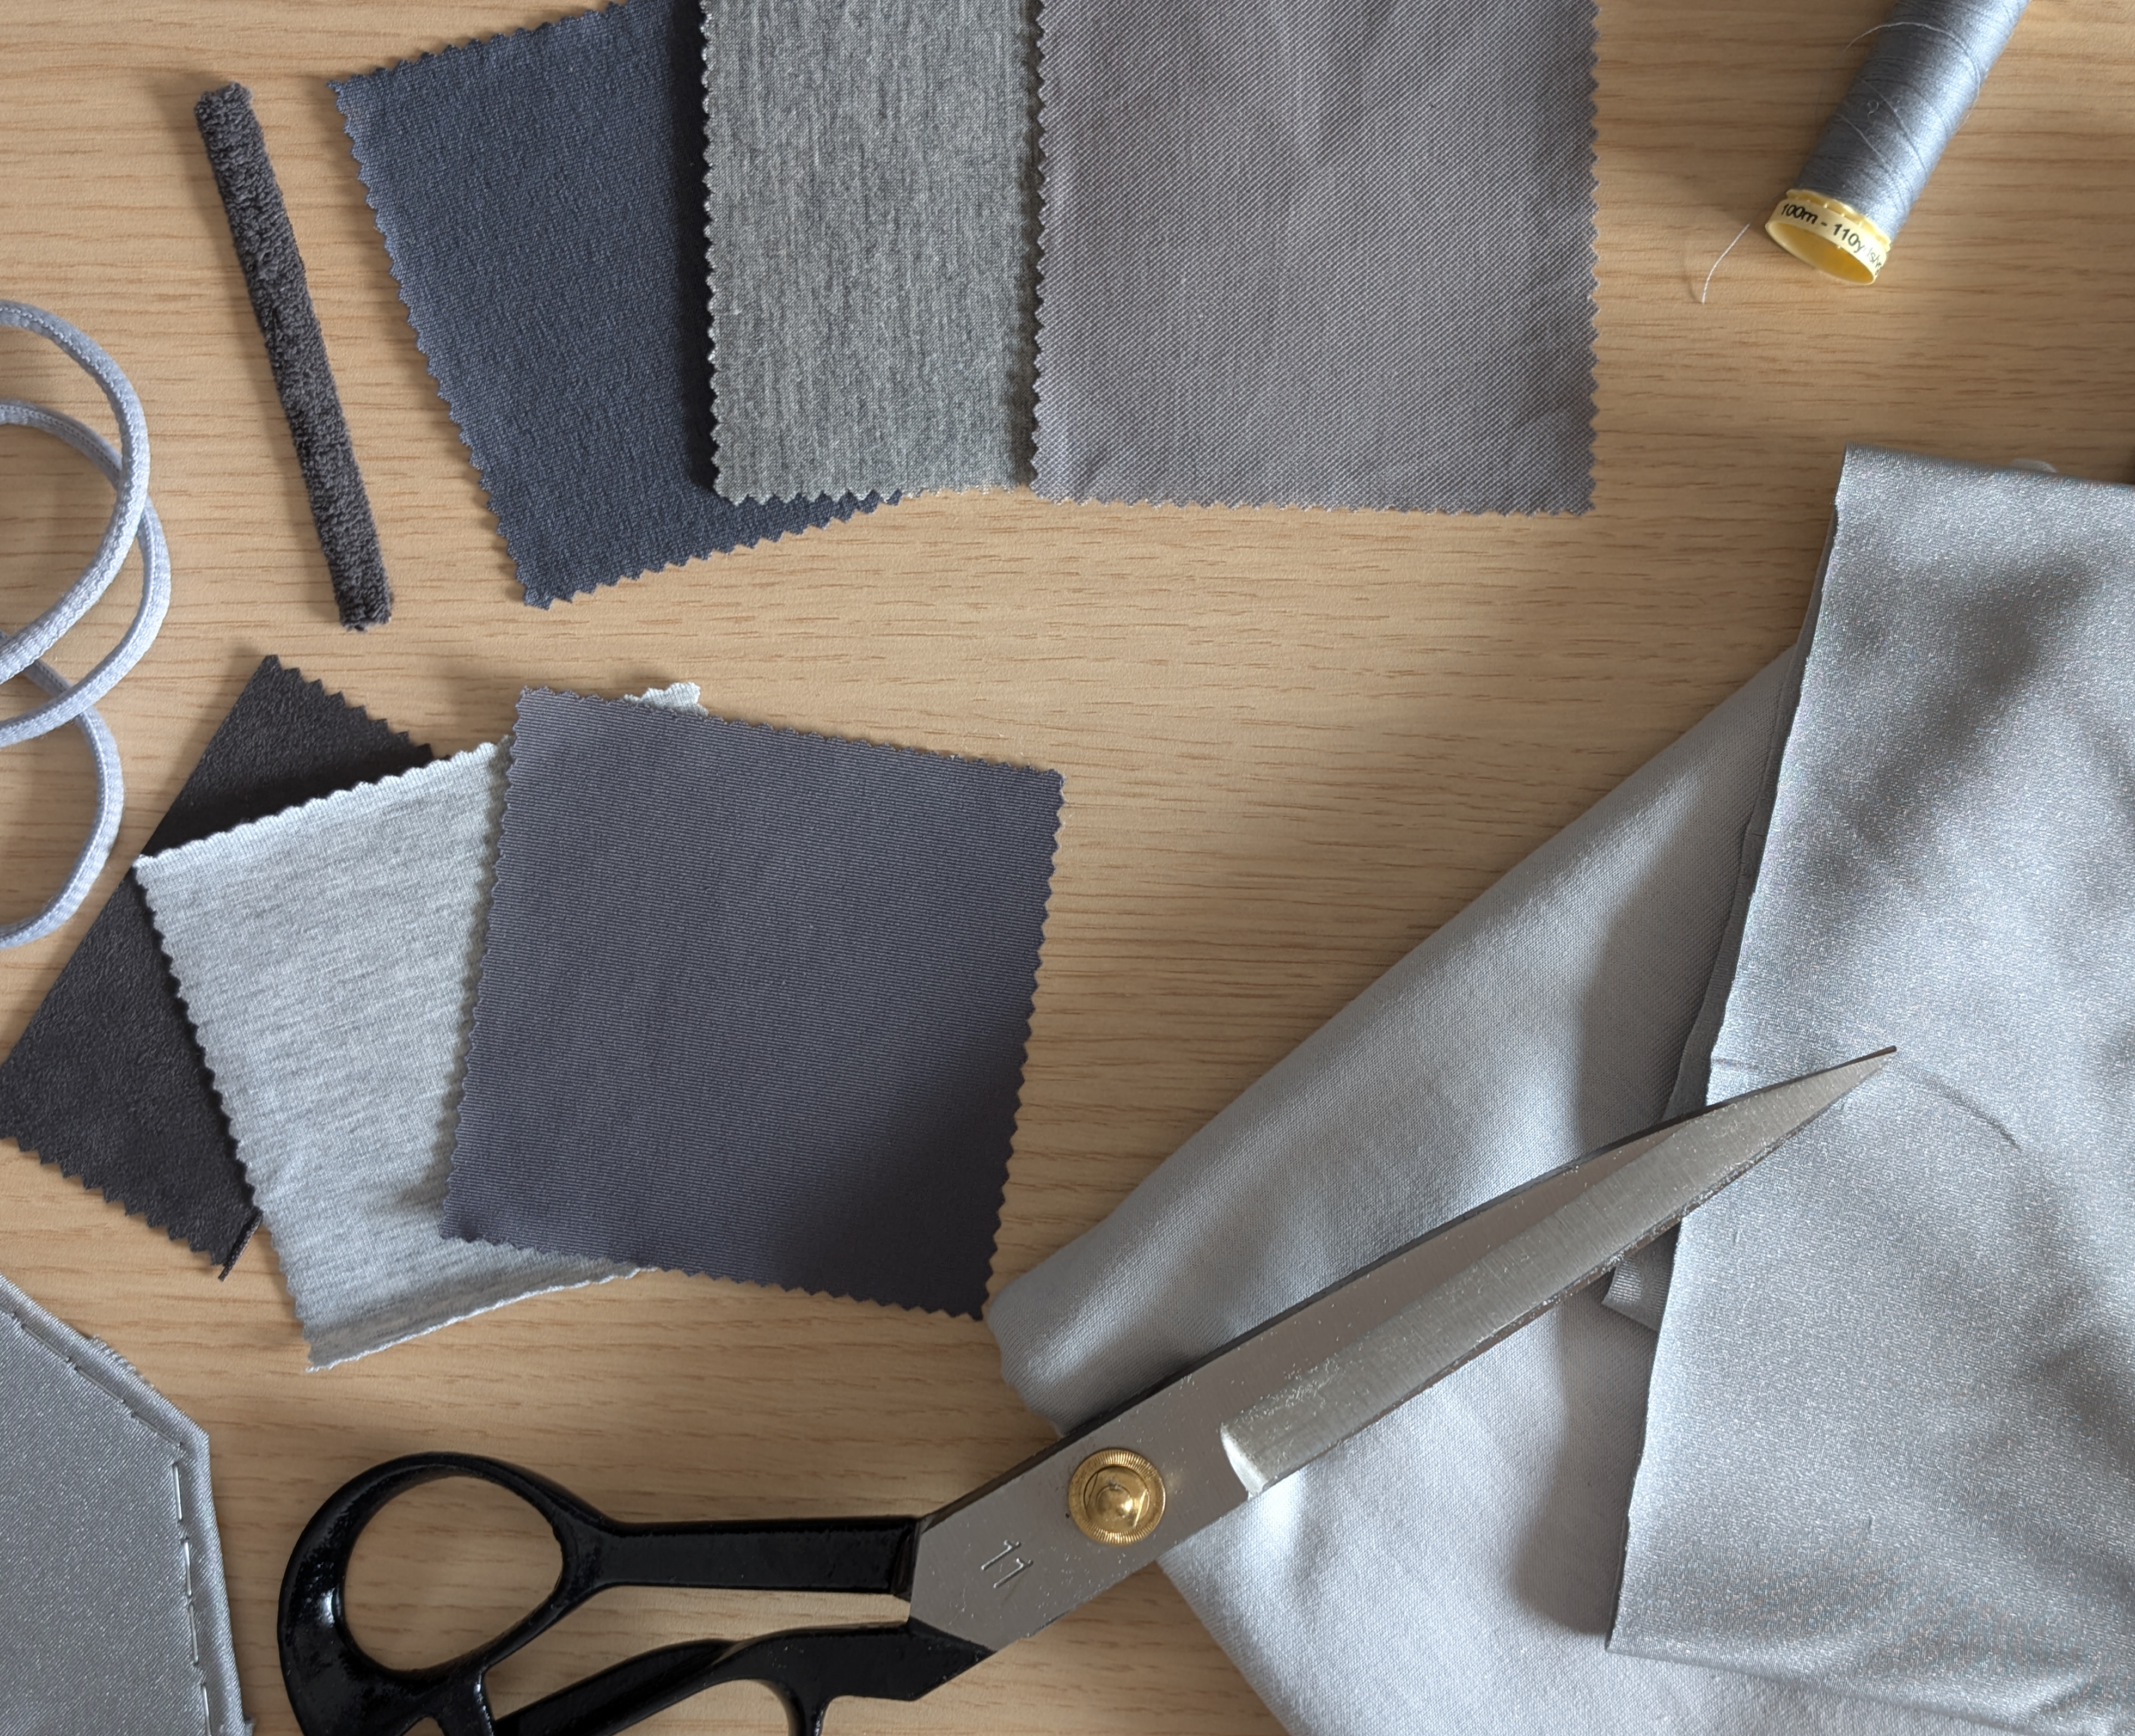
\includegraphics[width=1\linewidth]{images/Fabric Exploration.png}
    \caption{A broad sample of fabric was explored to identify a material that meets all requirements.}
    \label{fig:fabric-exploration}
\end{figure}

A separate, more detailed material exploration was conducted for the \textbf{volume slider} . While its long rectangular shape already affords a linear sliding gesture \cite{mlakar_design_2020}, the goal was to use the fabric itself to strengthen this affordance by leveraging the principles of signifiers \cite{mlakar_signifiers_2025}. 
% Guided by Mlakar et al.'s (2021) work, a \textbf{Textile Signifier} was created through material contrast. A cord fabric with a distinct directional nap was chosen for the slider. This "hairy" texture provides low resistance when swiped in the direction of the nap and higher resistance against it, strongly suggesting horizontal movement. 
Inspired by the principle that some textiles can create directional friction \cite{mlakar_exploring_2021}, a corduroy fabric with a distinct nap was selected. The fine "hairs" of the fabric were oriented to create a metaphor of resistance: sliding in one direction felt slightly different than sliding in the other, creating an intuitive link to the concepts of increasing and decreasing a value. This choice also created multiple layers of inherent feedforward cues. The texture itself acted as a \textit{Textile Signifier} \cite{mlakar_signifiers_2025}, creating a tactile and height contrast with the smooth base fabric, indicating the interactive nature of the slider, thus guiding the user where to interact. The nap also functioned as a \textit{Staging Signifier} \cite{mlakar_signifiers_2025}, as the unsettled portion of the fabric visually indicated the slider's current position and signified the direction it could be moved. Finally, several \textit{Visual Signifiers} \cite{mlakar_exploring_2021} were designed to reinforce the interaction, following the principle that users often assess an interface visually before touching it \cite{mlakar_exploring_2021, mlakar_signifiers_2025}. The slider was divided into sections that gradually increase in size from left to right, creating a clear visual metaphor for increasing a value (see Fig. \ref{fig:volume-slider-v1}). 
% While primarily affordance-clarifying, this graded division is also slightly function-revealing, though the specific function (e.g., volume) is not explicit from the form alone. 
This graded division adds a layer of function-revealing feedforward by clearly communicating the directionality of control. However, the cue remains generic, as it does not specify the particular function, such as volume, that is being adjusted. 
% The slider was given a darker color for visual contrast, a slightly slanted shape to emphasize horizontal motion, and internal divisions that gradually increase in size to afford the concept of "increase" toward the right.


\begin{figure}[H]
    \centering
    \includegraphics[width=1\linewidth]{images/Textile Prototype/Volume Slider V1.png}
    \caption{The volume slider design, using corduroy fabric to create directional friction. The gradually increasing segments act as a Visual Signifier for increasing a value from left to right.}
    \label{fig:volume-slider-v1}
\end{figure}


 The \textbf{pullable element for the "home" function} was realized as a physical cord, stitched into a loop. The loop shape acts as a strong signifier, inherently affording the action of being pulled up by a finger \cite{mlakar_signifiers_2025}. The loop expands over a width of approximately 45 mm, providing ample space for a finger to slide underneath, while the 5 mm diameter of the slightly squishy yet robust cord communicates durability. This element's state is also a key feedforward channel. Inspired by the concept of \textit{Staging Signifiers} by Mlakar et al. \cite{mlakar_signifiers_2025}, the loop's position indicates the system state. When a user navigates away from the main menu, a motor retracts the loop, making it flush with the surface and signifying that it can be pulled "up" again to return home (see Fig. \ref{fig:home-loop-v1}a). Conversely, when the main menu is active, the loop remains in its raised position (see Fig. \ref{fig:home-loop-v1}b), indicating that the action is complete and cannot be performed again.

 \begin{figure}[h!]
     \centering
     \includegraphics[width=1\linewidth]{images/Home Loop V1 small.png}
     \caption{The state of the "home loop" acts as a Staging Signifier. (a) In its retracted position, the loop signifies that it can be pulled up to open the main menu. (b) Once pulled, the loop remains raised while the main menu is active, indicating the action cannot be performed again.}
     \label{fig:home-loop-v1}
 \end{figure}
 

The \textbf{rotary dial} was implemented as a recessed circular groove with a depth of 3 mm (see Fig. \ref{fig:rotary-dial}), following recommendations from Nowak et al. \cite{nowak_shaping_2022}. This physical channel was designed not only to guide the user's fingertip for potential eyes-free use but also to visually afford a continuous circular motion, a principle supported by multiple studies \cite{dong_disappearing_2019, mlakar_design_2020, nowak_shaping_2022}. 
Within this dial, the central \textbf{tap surface} for confirmation actions was placed. This surface had a diameter of 35 mm as the comfort for the rotary gesture around it was prioritized. While a small enclosed shape generally affords a pressing gesture \cite{mlakar_design_2020}, it's size presented a potential pitfall as the surface is significantly larger than a fingertip. As Mlakar et al. \cite[pp.~1165]{mlakar_exploring_2021} pointed out; "If an element is circular and roughly the size of a fingertip, it affords pressing and will likely be assumed as a button [...]. If the circle is bigger, it becomes less clear whether the user is supposed to slide around the edge or press [...]”.  This potential ambiguity was to be validated in the subsequent user tests. To ensure this primary button was always locatable, its circular boundary was permanently marked with stitching, keeping it visible even when the surrounding dial groove was retracted and flush with the surface. 

\begin{figure}[h!]
    \centering
    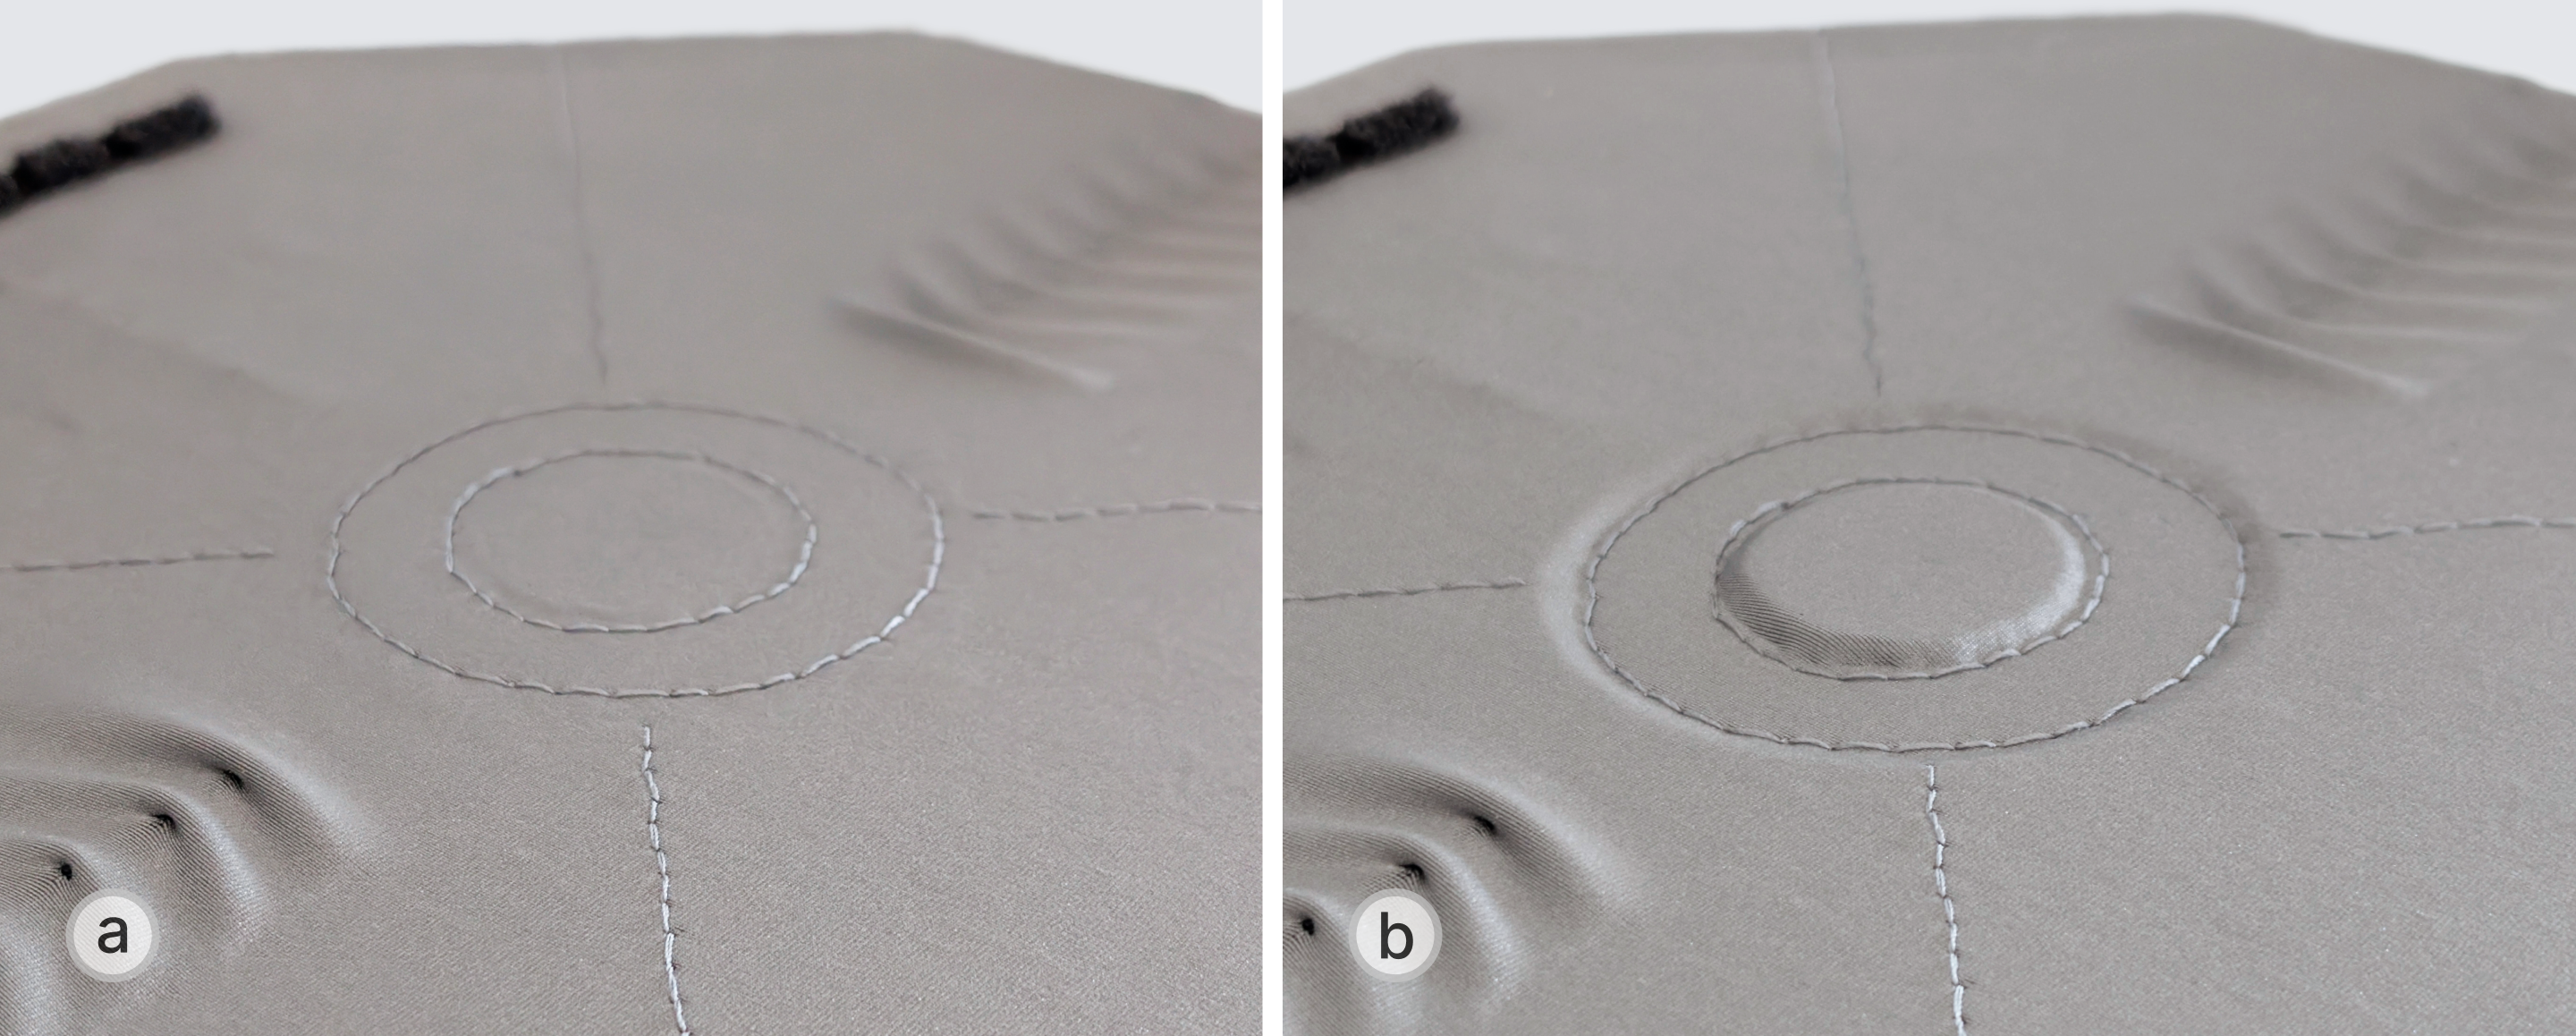
\includegraphics[width=1\linewidth]{images/Rotary Dial small.png}
    \caption{The shape-shifting rotary dial and central tap surface. (a) In its inactive state, the dial is flush with the surface, with permanent stitching marking the boundary of the tap area. (b) When active, the dial forms a recessed groove to guide the user's finger in a continuous circular motion.}
    \label{fig:rotary-dial}
\end{figure}

% The central confirm/select function was designed as a large tap surface with a 35 mm diameter, located within the rotary dial. Following the principle that a circle roughly the size of a fingertip affords pressing, this large surface was designed to afford a simple tap, without requiring the system to distinguish between different numbers of fingers. The circular outline of this tap area remains permanently visible via its stitched border, even when the rotary dial's groove is hidden.

The \textbf{directional swipe areas} make significant use of the fabric's deformability to create clear, unambiguous cues. The design goal was to create a surface that specifically affords a swipe in one direction only. To achieve this, a pleating texture was chosen, as this has been found to be a strong signifier for stroking or stroking gestures \cite{jiang_gesfabri_2022} (see Fig. \ref{fig:directionaö-swipe-areas-v1}c). 
However, to clarify the directionality, the shape-shifting mechanism itself was designed as a story telling \textit{Staging Signifier} \cite{mlakar_signifiers_2025}. The pleats are formed by pulling the fabric from underneath along a straight line of pulling-points; the observable direction of this tension indicates the intended gesture path. This also creates a \textit{Visual Signifier} \cite{mlakar_signifiers_2025}, as the pleats have a slightly pointy character, akin to an arrow (see Fig. \ref{fig:directionaö-swipe-areas-v1}b), indicating the intended direction of interaction \cite{mlakar_exploring_2021}. Based on an analysis of the system's functionalities, it was noted that the left and right directional swipes are always used as a pair; therefore, their corresponding pleats were connected to a single motor to appear and disappear together. The top swipe surface, however, is activated independently by a separate motor as needed.

\begin{figure}[h!]
    \centering
    \includegraphics[width=1\linewidth]{images/Directional Swipe Areas V1.png}
    \caption{The directional swipe areas in their two primary states. (a) A completely flat plane for 2D pointing tasks. (b, c) When activated, the fabric forms pleated guides that serve as visual and tactile signifiers for a directional swiping gesture.}
    \label{fig:directionaö-swipe-areas-v1}
\end{figure}

% Finally, a deliberate decision was made regarding the large \textbf{2D plane used for pointing tasks} (e.g., the POI or soundscape applications). No additional inherent physical cues were added for this mode, as they could interfere with the tactile cues of the other elements when the surface is in a different state. For this specific function, the system relies on the visual feedforward from the WSD's graphical user interface to suggest and guide the pointing interaction. This is a common strategy when a single physical surface must support multiple, distinct interaction models.

Finally, for the large \textbf{\gls{2D} pointing plane} used in tasks like the \gls{POI} selection, a conscious decision was made to not add any permanent inherent cues like a grid texture (see Fig. \ref{fig:directionaö-swipe-areas-v1}a). This was to avoid creating conflicting tactile information that could interfere with the other dynamic elements when they are active on the same surface. 
Instead, the design relies on two sources of feedforward: visual guidance from the \gls{WSD}'s \gls{GUI} to suggest the pointing task, and the inherent affordance of the surface itself. 
It was hypothesized that a completely flat and uniform plane could naturally communicate that the entire area is a single, continuous space available for interaction, an assumption to be evaluated in the subsequent user tests. 

Across all of these elements, two overarching principles guided the design. First, following the recommendation to design all shapes as simple as possible \cite{mlakar_design_2020}, the interactive zones were based on simple geometric forms like circles and lines. Second, a principle of economical use of signifiers was applied. While multiple layers of cues (Visual, Textile, and Staging) were often combined to strengthen an affordance, care was taken to avoid redundancy and unnecessary complexity, in line with suggestions that an "economic usage" of signifiers leads to better understanding of the interface \cite{mlakar_exploring_2021, mlakar_signifiers_2025}. The ultimate goal of this clear and economical design approach was to create perceptible affordances that were unambiguous to the user, thereby avoiding the usability pitfalls of hidden or false affordances \cite{gaver_technology_1991}.

\subsubsection{Designing the \gls{WSD}'s Graphical User Interface (\gls{GUI})}

The design of the \gls{WSD}'s Graphical User Interface (\gls{GUI}) was guided by the philosophy of creating an unobtrusive system that seamlessly integrates with the vehicle's interior and the outside view. The goal was to avoid a visually disjointed or "stuck-on" feeling, instead crafting a soft, organic interface that aligns with the "living space" concept and feels like a natural part of the environment.

\begin{figure}[h!]
    \centering
    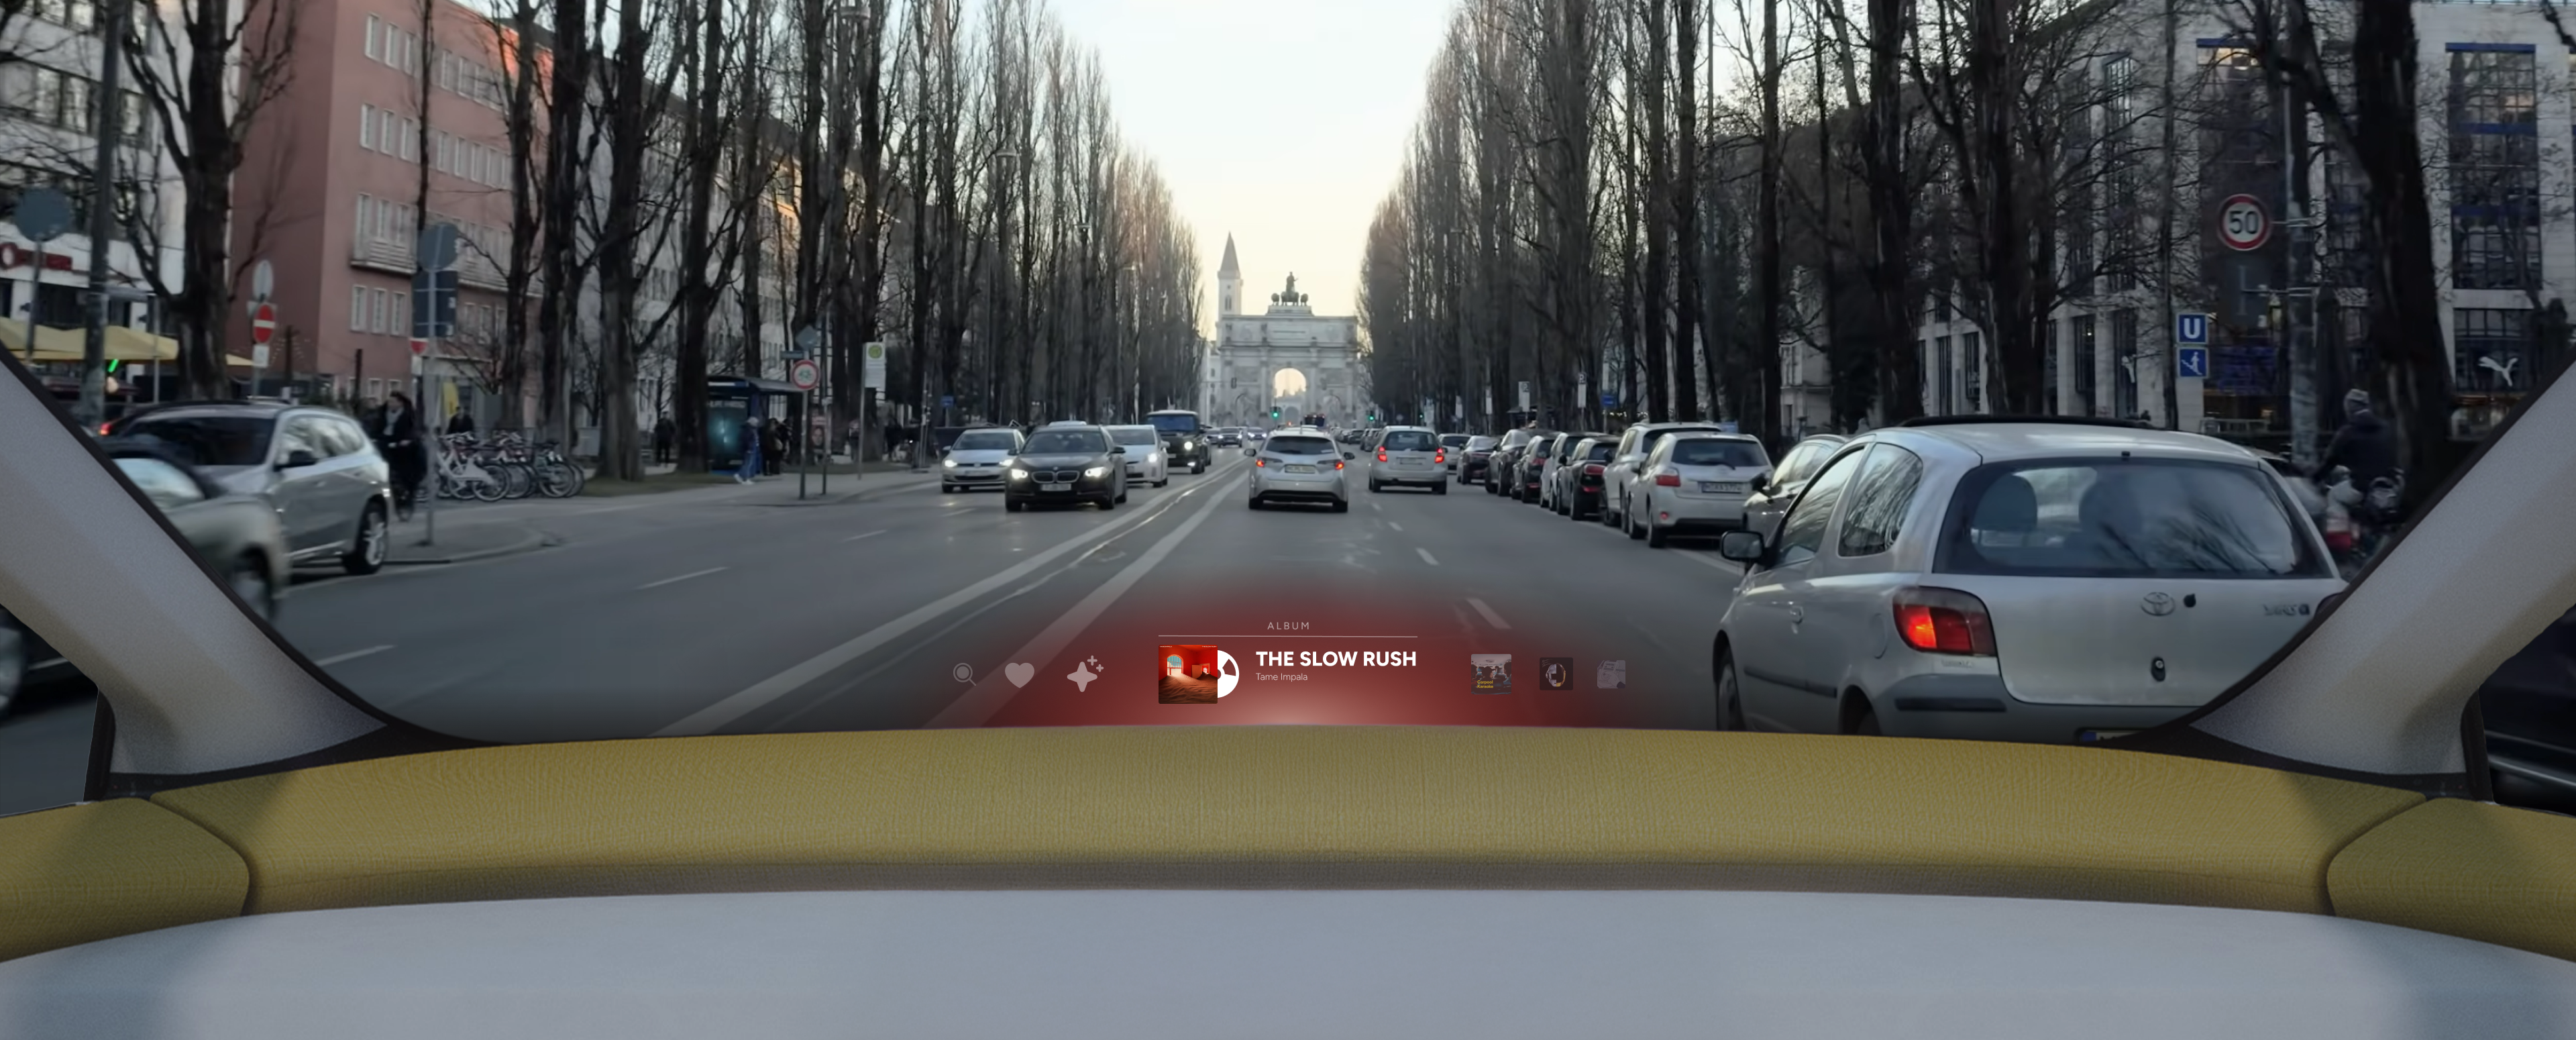
\includegraphics[width=1\linewidth]{images/Music - THE SLOW RUSH.png}
    \caption{Music Player Application, Example to show the UI located at the bottom of the \gls{WSD}, as to not obstruct the view.}
    \label{GUI-location-WSD}
\end{figure}


The layout and information hierarchy were designed to be intuitive and to complement the physical textile controller. The majority of \gls{UI} elements are displayed centrally at the bottom of the \gls{WSD}, appearing to hover over the vehicle's dashboard (see Fig. \ref{GUI-location-WSD}). This placement ensures that the \gls{GUI} occupies the view of the road immediately ahead but does not obstruct the user's view of the surrounding landscape. While research has shown a preference for landscape-oriented windows \cite{riegler_augmented_2019}, the design abandoned hard rectangular shapes in favor of soft, rounded, and elliptical forms. These shapes gradually fade into the background at the edges, creating a less intrusive feel. A core principle was maintaining a strong \textbf{spatial mapping} between the on-screen layout and the physical textile interface. For example, in the home menu (see Fig. \ref{fig:GUI-layout-examples}a), the centrally highlighted menu item corresponds to the central tap surface, while other items are arrayed horizontally around it, aligning with the left and right directional swipe areas. This principle is also evident in selection prompts, where options appear as movable "marbles" around a central selection (see Fig. \ref{fig:GUI-layout-examples}b); the user physically swipes the desired marble into the center of the screen, mirroring the action on the textile surface. Likewise, when the rotary dial is active, \gls{UI} elements are arranged in a circle, such as the contacts list that emulates a rotary phone (see Fig. \ref{fig:GUI-layout-examples}c) or the image of a vinyl record in the music player that can be "spun" to seek through a track (see Fig. \ref{fig:GUI-layout-examples}d).


\begin{figure}
    \centering
    \includegraphics[width=1\linewidth]{images/GUI-layout-examples.png}
    \caption{\gls{GUI} design samples illustrating the system's core interaction metaphors: (a) horizontal list navigation in the home menu, (b) the "marble" selection metaphor, (c) a rotary layout for the contacts list, and (d) the "spinning vinyl'" metaphor for media control.}
    \label{fig:GUI-layout-examples}
\end{figure}


The visual design was crafted to be both aesthetically pleasing and highly functional. Instead of solid colors, the background of each application consists of soft gradients, rather than solid colors, that reflect the dynamic blending of colors of the scenery outside the \gls{WSD}, with each application having a unique gradient for clear identification. These gradients are also dynamic; for example, accepting a call by selecting the green "marble" causes the background to bloom into a corresponding green gradient as feedback, indicating a now active call. 
To maintain legibility while blending with the environment, all background elements had an 80\% opacity that faded out at the edges. To ensure contrast against varying external conditions, this was overlaid on a semi-transparent black background field (40\% opacity), a practice supported by the findings of Riegler et al. \cite{riegler_adaptive_2019}. 
% The main GUI elements are rendered at 80\% opacity and fade at the edges, supported by a semi-transparent (40\% opacity) black background area that also fades out, ensuring legibility without being obtrusive, in line with findings from Riegler et al. (2019). 
Typography was built on a clear hierarchy using the sans-serif font Figtree \cite{kennedy_figtree_nodate}. Prominent text is bold, while secondary information uses variations in font weight and transparency. All text is white to maintain contrast against the dynamic backgrounds. For iconography, the clear, minimalist, open-source Phosphor icon pack \cite{fried_phosphor_nodate} was used.

Finally, motion design was a critical channel for feedforward, used to make the interface feel alive and to guide interaction. The very first interaction on the welcome screen is a pulsing circles designed to look like water ripples (see Fig. \ref{fig:welcome+spotlight}a), directly mirroring the circular stitching on the physical prototype and affording a touch to "start" the system. Other dynamic cues were used throughout: the selected item background in the main menu has a subtle "breathing" animation to afford a tap; the "marbles" in a selection prompt animate from the center outwards when they appear, showing their potential trajectory back to the center; and when opening an album in the music player, the vinyl record icon animates out of the album cover art with a slight spin, suggesting the rotational gesture that controls it. 
Similarly, for the \gls{2D} pointing task in the Point of Interest (\gls{POI}) function, a spotlight-shaped cursor (see Fig. \ref{fig:welcome+spotlight}b) appears and subtly moves around the center of the screen, mimicking an eye scanning the scenery. This initial, autonomous movement acts as a critical feedforward cue, signifying that the cursor is a dynamic, draggable element that the user can control, rather than a static icon.
% These microinteractions were designed to make every touch feel responsive and to intuitively communicate how the interface could be used.

\begin{figure}[h!]
    \centering
    \includegraphics[width=1\linewidth]{images/Welcome+Spotlight.png}
    \caption{The use of dynamic cues as feedforward to guide interaction. (a) A pulsing ripple animation on the welcome screen invites a "start" touch. (b) The autonomous movement of the spotlight cursor upon opening the app signifies its draggability for selecting the nearby POI.}
    \label{fig:welcome+spotlight}
\end{figure}

These dynamic cues were part of a broader strategy to follow the principles of a Natural User Interface, or \gls{NUI} \cite{wigdor_brave_2011}, where every physical interaction elicits an immediate, corresponding, and natural-feeling reaction from the \gls{GUI}. For example, turning the physical dial causes the on-screen element to rotate accordingly, and swiping a "marble" on the textile surface results in its digital counterpart fluidly moving into the central selection zone, making the tangible interaction feel both intuitive and directly manipulative. 

\subsubsection{Defining Feedforward Levels for Evaluation}
% This is the perfect place to explain the 'why' and 'what' of your study's core conditions, as you have just defined the baseline: Inherent Cues.

To systematically investigate the research gap concerning intuitive interaction, three distinct levels of feedforward were defined for evaluation. This approach allows for a controlled comparison, as each level builds upon the same physical prototype and baseline \gls{GUI}. The conditions were not chosen at random; they were deliberately designed to represent three distinct and representative points on the Feedforward Matrix, spanning a spectrum from purely physical, inherent cues to progressively more augmented and function-revealing forms of guidance (see Fig. \ref{fig:success-rates-condition}). This strategy allows for a meaningful analysis of how different feedforward philosophies impact the user experience.

\begin{figure} [h!]
    \centering
    \includegraphics[width=1\linewidth]{images/Feedforward Matrix/Feedforward Matrix Conditions V2.png}
    \caption{Feedforward Matrix, visualizing the feedforward conditions: (a) Inherent Cues, (b) Augmented Light Cues, and (c) Augmented Text Cues.}
    \label{fig:feedforward-matrix-conditions}
\end{figure}

\paragraph{Condition 1: Inherent Cues (Baseline):}

This condition represents the purest form of physical guidance and serves as the experimental baseline. It relies solely on the inherent feedforward cues designed into the prototype's physical form, as detailed in the previous section \ref{inherent-feedforward}. Users receive guidance only from the shape, texture, position, and deformability of the textile elements.

On the Feedforward Matrix, this condition occupies the top-left end of the axes (see Fig. \ref{fig:success-rates-condition}a). Its cues are fully embedded in the material and are almost exclusively Affordance-Clarifying, designed to answer the question, "What can I do and how?" through tactile and physical properties alone.

\paragraph{Condition 2: Augmented Light Cues:}
This condition explores a subtle, seamlessly integrated layer of augmentation by adding dynamic light projections directly onto the textile surface. A key strength of these projections is the ability to reinforce the directionality of an interaction through subtle animations that guide gestures, clarifying how to interact. For instance, soft swipe animations moving along the physical pleats of the directional swipe areas add another layer of guidance on top of the inherent physical cues (see Fig. \ref{fig:arrow-dial-lc}). The light cues also allow for easy integration context-dependent affordances. For example, while the physical rotary dial affords rotation in both directions, a light animation, such as a glowing circle accelerating repeatedly in one direction, can signify that, in the current context (e.g., at the beginning of a list), only a single direction of rotation is possible.


\begin{figure}[h]
    \centering
    \includegraphics[width=1\linewidth]{images/ArrowDialLC.jpg}
    \caption{The seamlessly integrated augmented light cues during music playback. Animated arrows on the pleated surfaces guide swipe gestures, while a rotational cue on the dial affords playback control.}
    \label{fig:arrow-dial-lc}
\end{figure}

% Beyond these affordance-clarifying abilities, the light cues also have potential to hint at the interaction's function through the use of color, creating a direct visual link to UI elements on the WSD. This allows for easy mapping between the GUI and the physical controls, clarifying what a gesture will result in. For instance, the light projected onto the three directional swipe areas would match the colors of the corresponding "marble" options displayed on the screen. Critically, the light projections also serve to establish the initial connection between the WSD and the textile controller for a first-time user. On the welcome screen, the pulsing "water ripple" animation on the WSD is mirrored by a light projection on the textile surface, strongly affording a touch in the center while simultaneously linking the two interfaces.

Beyond clarifying affordances, the light projections also served to communicate the system's current state and the availability of controls. While the dynamic elements on the textile surface use shape-shifting to signal their availability, the light projections add this dynamic layer to the static elements, such as the volume slider and home loop. The light can display the current state of a control, for example by illuminating a portion of the slider to represent the current volume level. It can also signify when a static element is interactive; the volume slider and home loop are only augmented by light when their functions are available in the current context, e.g. when there is active media playback. Furthermore, the use of dynamic color creates a direct visual link to \gls{UI} elements on the \gls{WSD}, which serves a function-revealing purpose by allowing for easy mapping between the \gls{GUI} and the physical controls. For instance, the light projected onto the three directional swipe areas would match the colors of the corresponding "marble" options on the screen (see Fig. \ref{fig:marble-lc}), clarifying the result of a user's action. Critically, the light projections also serve to establish the initial connection between the \gls{WSD} and the textile controller for a first-time user. On the welcome screen, the pulsing "water ripple" animation on the \gls{WSD} is mirrored by a light projection on the textile surface, strongly affording a touch in the center while simultaneously linking the two interfaces.

\begin{figure}[h]
    \centering
    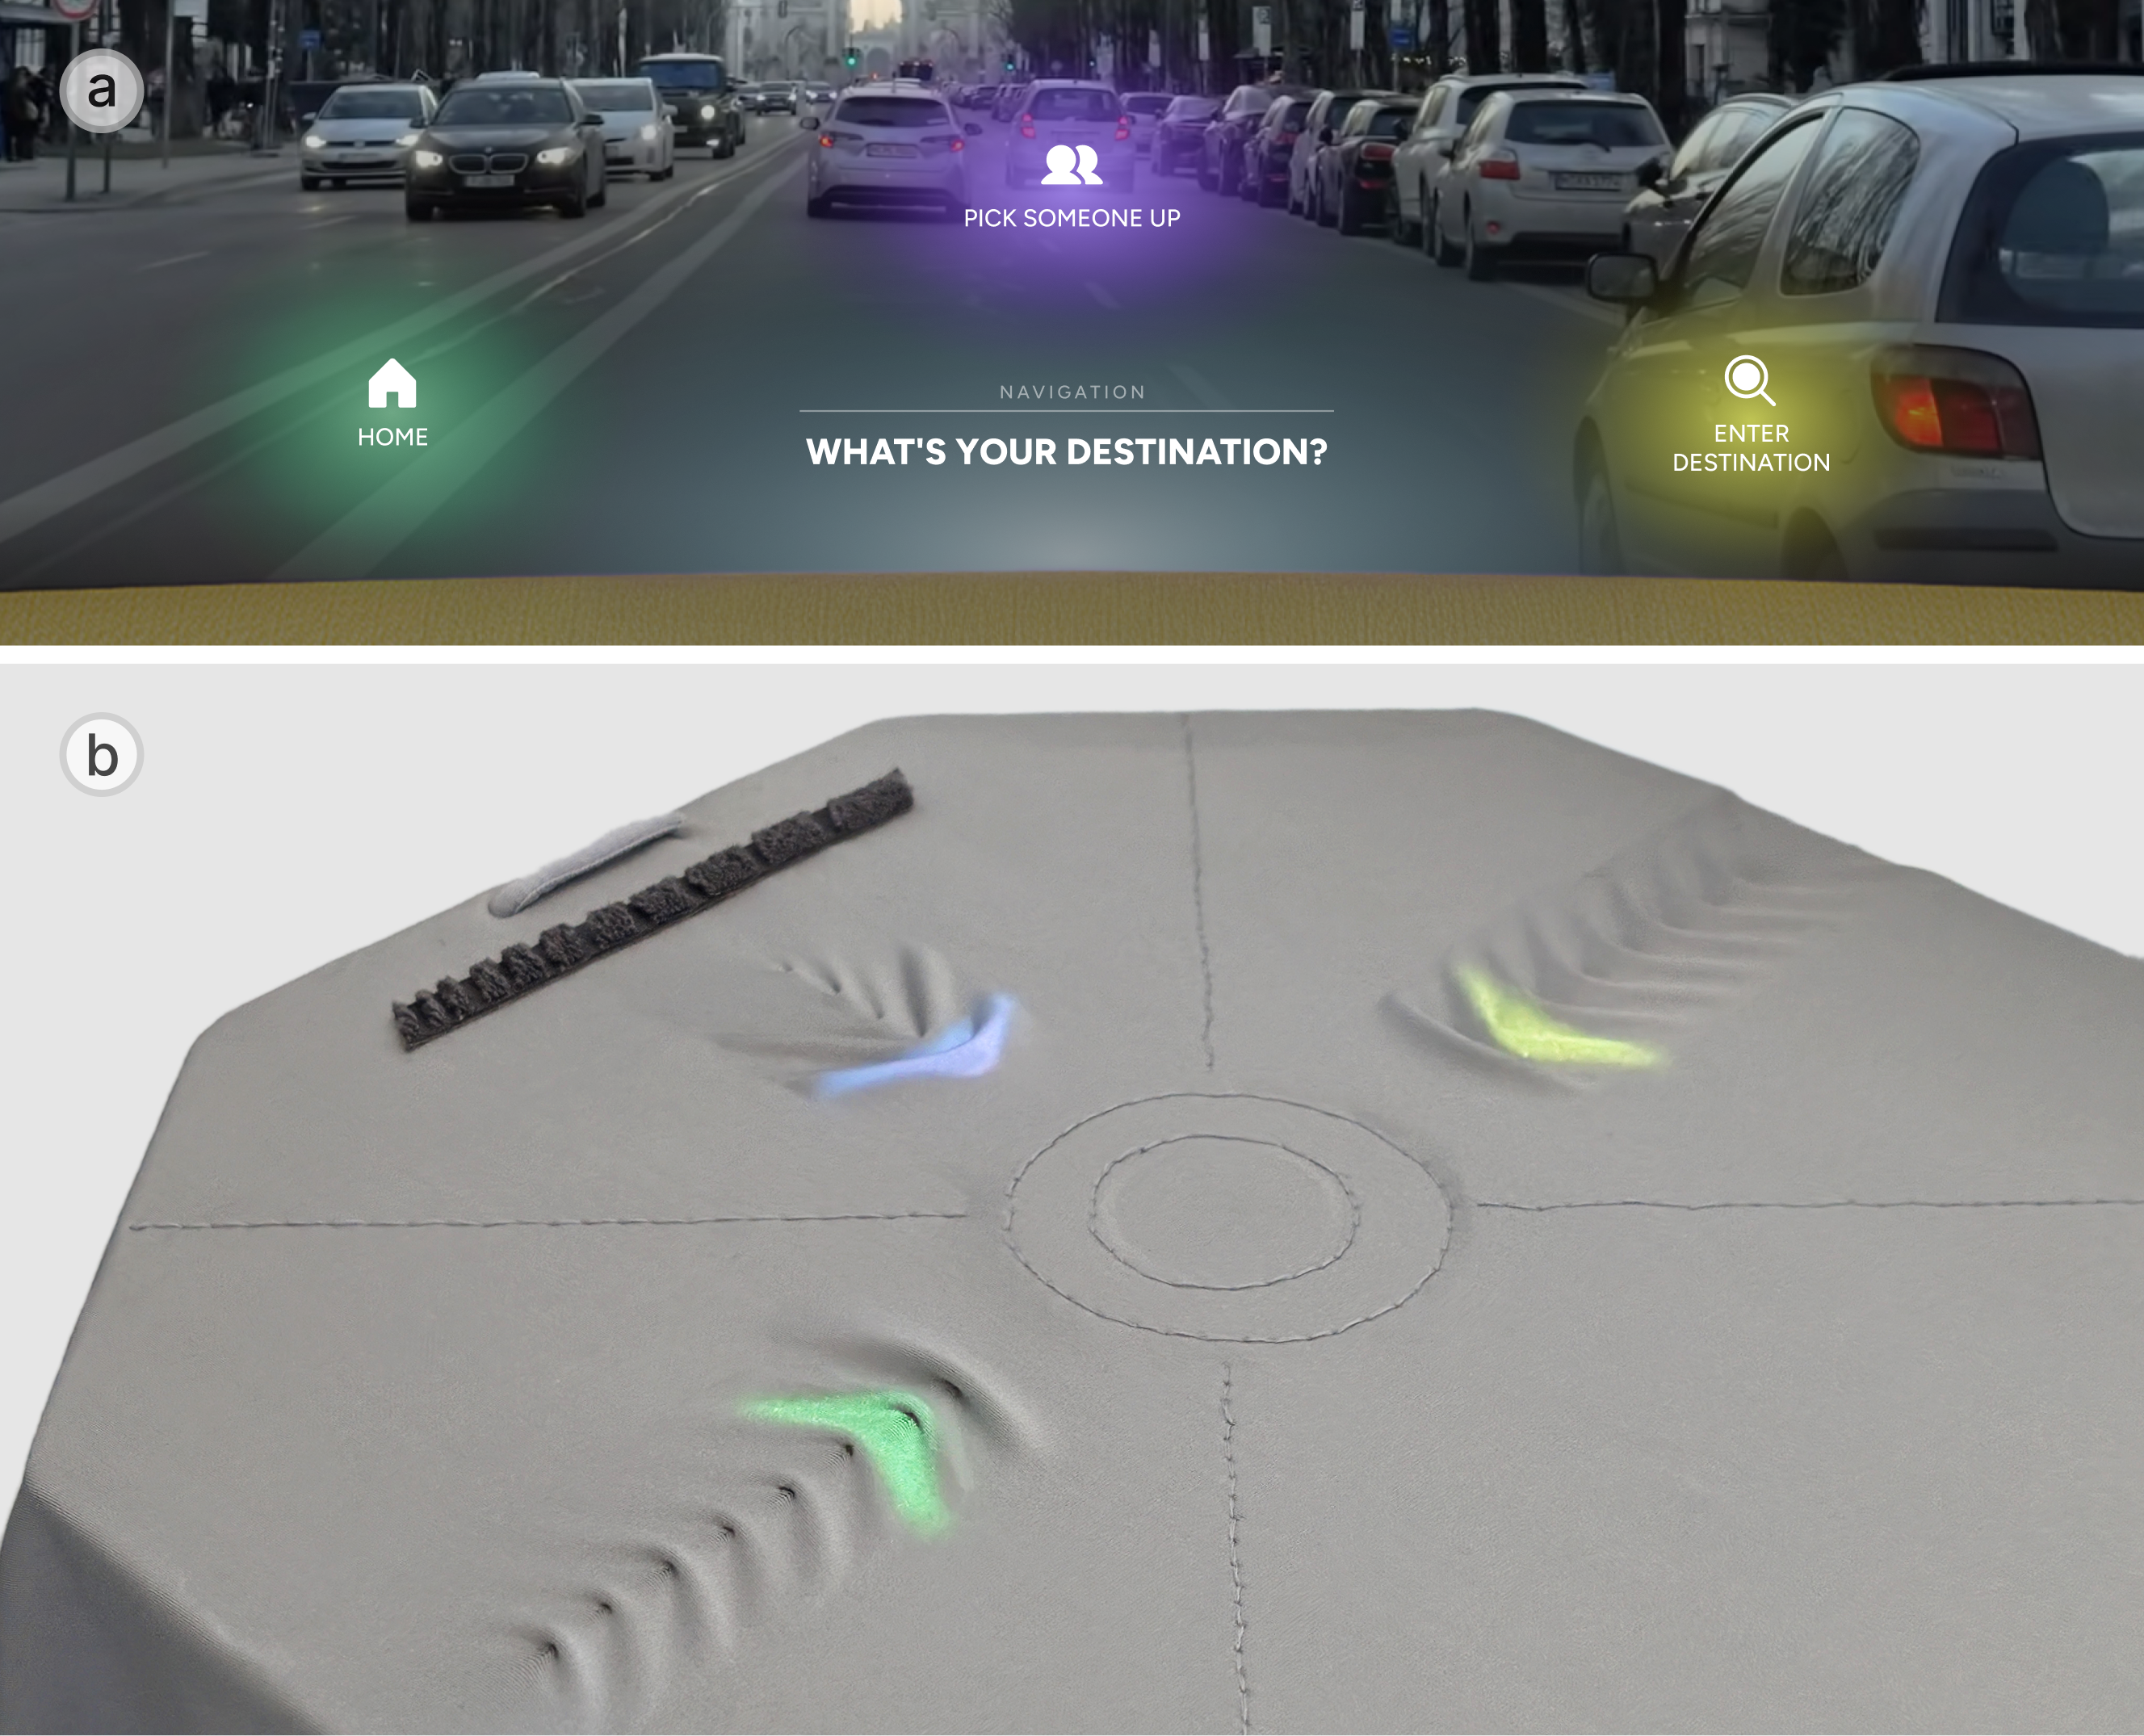
\includegraphics[width=1\linewidth]{images/Marble LC.png}
    \caption{The use of color-coded light cues to create a direct function-revealing mapping between the GUI and the physical interface. During the "marble" selection task, the colors of the on-screen options (top) directly correspond to the light projected onto the interactive textile areas (bottom).}
    \label{fig:marble-lc}
\end{figure}

The visual design of these cues aimed for a "shy" integration, with blurred edges, smooth animations, and projected shapes that precisely follow the physical form of the elements, allowing them to seamlessly blend into the fabric. On the Feedforward Matrix (see Fig. \ref{fig:success-rates-condition}b), this condition sits between fully Embedded and Augmented, leaning more towards Embedded due to its seamless integration. Informationally, it is mostly Affordance-Clarifying but also introduces Function-Revealing elements through its color mapping.


\paragraph{Condition 3: Augmented Text Cues:}
This condition investigates the effect of explicit, textual instruction by adding written hints directly into the \gls{WSD}'s \gls{GUI}. The aim was to be as unambiguous as possible about both the required action and its resulting function.

To integrate these cues in a predictable yet unobtrusive manner, they were given a single, consistent position at the bottom of the \gls{GUI} (see Fig. \ref{fig:text-cue-examples}). This placement ensures that a user seeking guidance always knows where to direct their gaze. The instructions followed a consistent formula, clearly stating which gesture leads to which function (e.g., "Tap to view forecast", "Swipe left to decline"). A key design challenge was balancing the need for these cues to be short and easily graspable with the risk of ambiguity that can arise from oversimplification. Another challenge was avoiding information overload in complex situations with multiple interaction possibilities, such as during playback in the media player. To solve this, a maximum of two cues were displayed side-by-side (see Fig. \ref{fig:text-cue-examples}b); if more instructions were needed, they would fade in and out in timed intervals to avoid overwhelming the user.

\begin{figure}[h]
    \centering
    \includegraphics[width=1\linewidth]{images/Text Cues Examples.png}
    \caption{Examples of the augmented text cues, designed for clarity and predictability. The cues appear in a consistent location at the bottom of the screen (a), with a maximum of two displayed side-by-side to explain multiple interaction possibilities, like an incoming call (b).}
    \label{fig:text-cue-examples}
\end{figure}

On the Feedforward Matrix (see Fig. \ref{fig:success-rates-condition}c), this condition is positioned towards the Augmented/External end of the integration axis, as the cues are integrated in the \gls{GUI}, physically distant from the textile controller. Informationally, it is a mix of Affordance-Clarifying (e.g., "spin clockwise") and Function-Revealing (e.g., "to fast-forward"), with a stronger emphasis on revealing the function, as the textual description of a gesture is more abstract than a physical or seamlessly integrated visual cue directly mapped on the surface.

% +++++++++++++++++++++++++++ ADD CONDITION MATRIX HERE +++++++++++++++++++++++++++++++++++++

\subsubsection{Scenario Selection and Storyline Creation}

\paragraph{Defining the Scope of the Study:} \mbox{} \\
From the full set of designed \gls{NDRA}s, it was necessary to select a representative subset for full implementation in the user study prototype. The primary criterion for this selection was the need to maximize the diversity of interaction types to ensure that the full range of the prototype's capabilities was thoroughly evaluated. Specifically, the selection was guided by the need to include examples of all the core interaction primitives designed for the textile surface: simple \textbf{taps} for selection, \textbf{linear continuous input} (volume slider), \textbf{rotary continuous input} (dial), \textbf{directional swipes} for choices and menu navigation, the textile-specific \textbf{pull gesture} for the home menu, and the \textbf{\gls{2D} pointing plane}.

To cover these varied interactions, a set of functions and applications was chosen for implementation. This included an essential ride-starting sequence composed of a \textbf{welcome screen} and \textbf{navigation prompts} (for destination and route confirmation). In addition, a suite of common in-vehicle applications was implemented, reflecting some of the most frequently cited \gls{NDRA}s for future \gls{AV}s. This selection included a \textbf{Music Player} to support leisure and entertainment needs \cite{ahram_what_2020, large_design_2017, pfleging_investigating_2016, wilson_non-driving_2022},  and a \textbf{Phone/Call system} with contacts and messaging to support the critical roles of communication and productivity \cite{ahram_non-driving_2020, large_design_2017, pfleging_investigating_2016, wilson_non-driving_2022}. Finally, the novel \textbf{\gls{POI} Spotlight application} was included to directly enhance the common activity of looking out the window \cite{berger_designing_2021, ahram_what_2020, pfleging_investigating_2016, stampf_deriving_2024} by augmenting the view with enriching information, a key potential for \gls{WSD}s identified in the literature \cite{berger_designing_2021, haeuslschmid_first_2016, matsumura_active_2018, pagura_window_2011}. This curated set of tasks ensured that every designed interaction primitive would be evaluated within a contextually relevant and well-justified application.

\paragraph{Creating the User Experience:} \mbox{} \\
\begin{comment}
% A cohesive storyline connecting these interactions into four distinct scenarios ("Welcome", "Music", "Spotlight", and "Call") was created.
% This narrative approach was designed to help participants in the user test vividly imagine the context of use and experience the prototype in a more immersive and engaging way. The main story line is that the participant is that they finished work and got to their car (a fully autonomous vehicle SAE level 5) in the parking lot. they now want to drive home.
% Scenario 1: Welcome: The journey begins with the 'Welcome' scenario. Upon entering the vehicle, the user is presented with the pulsing ripple on the \gls{WSD}, prompting their first interaction to 'start' the system. after that the system guides the user through a precess to start the drive with the AV, asking for the destination (participant has to select the home destination) then which route (user is free to choose from fastest, eco and scenic) and then view an overview of the journey ahead and confirm it to start the right. this introduction process that is required to start the drive with the vehicle as there are no manual driving controls on the other hand it is designed to carefully introduce the system to novice users without being annoying or slowing down expert users. for this we used the scaffolding design principle for NUIs proposed by Widgor and Wixon 2013. This prinicpile's goal is  "is that the user moves from "novice" to "expert" quickly and with pleasure. By novice we simply mean someone who uses the system for the first time. By expert we mean someone who uses the system in the way that the designers intended, feels pleasure in those activities, and has achieved that level of competence without the slow and tortuous learning that is typical of mastering many new interfaces".
% This scenario tests the crucial first steps of discoverability and walk-up-and-use(ability) since there is no explicit tutorial or onboarding teching process before the user can use the system (like that was the og research goal).
% Scenario 2: Music: After starting the drive home, the narrative continues with the user deciding to play music. The user is given a specific album name to find and to start playback of a song. Here another example of scaffolding can be found as upon opening an album the playback of the first song does not start immediately, however the user first has to give the vinly record displayed on the WSD a spin to start playback introducing the user to the methaphor and teaching that the rotary dial in this application is used to physically move the vinyl, thus allowing for interactions like fast forwarding or rewinding based on the spin direction, as well as pausing the playback by holding down the record, physically stopping it's movement and thus the playback. After starting the playback other tasks in this scenario include changing the volume, seeking in the song, skipping a song. Then the user does not feel like music anymore so they pausing the playback and returning back to the home menu.  idk what this scenario was made for in ters of what it can find out, i guess it's an example of a playful unconventional interaction methaphor from a music player which might have a good positive experience but also risks to be dificult to understand, however as described earlier one of the goals when design  the interface are these playful interactions and avoiding of just replicating interaction on the textile interface from it's digital counterparts.
% Scenario 3: Spotlight (POI): the vehicle is in some dense traffic with little movement, but since the user has not been in this part of town before they want to find out more about their surrounding, so they open  the 'Spotlight' application, it shows a total of three POI which can be selected by dragging the spotlight cursor around on the 2D pointing plane,. when the cursor gets close to POI it snaps onto the POI and after a short dwell time it opens a window with informations about the location like it's name, fun facts and opening times. int he scenario the user is interested to find out more about two buildings, after getting the information they leave the application and return to the home menu. idk what this scenario evaluates.
% Scenario 4: Call: "Finally, the user receives an incoming phone call from a coworker, they accept the call and get to know that the coworker has to cancel a meeting that was scheduled for tomorrow morning, they remember that another coworker called Daniel was also invited and ask the user to send them a short message letting him know the meeting is canceled , while the person on the phone says this the system is actively listening and giving the user matching information about the scheduled meeting. the person on the phone hangs up and the user has to message Daniel without further guidance. this requires opening the contacts lit, navigating through it with the rotary dial and finding and selecting daniel, the system displays infromation from the call the user just had signifying that the meeting with daniel should be cancled through a message, then through a series of promts the user can choose to send a message and sees two examples written by the system, they can choose any of their liking, after the message is sent they return to the home menu. This scenario was intentionally deigned to review all previously used interactive elements on the textile interface (except for the volume slider) but presenting these in diferent context, this is to evaluates if the user has sucessfully learned how the system works.
\end{comment}
To evaluate the prototype, a cohesive storyline was created that connects the various interactions into four distinct scenarios. This narrative approach was designed to help participants vividly imagine the context of use and experience the prototype in a more immersive and engaging way. The storyline places the participant in a fully autonomous, SAE Level 5 \cite{on-road_automated_driving_orad_committee_taxonomy_2021} vehicle after finishing work; their goal is to start a journey and drive home.

\subparagraph{Welcome Scenario}
The journey begins with the Welcome Scenario. Upon entering the vehicle, the user is presented with the pulsing ripple on the \gls{WSD}, prompting their first interaction to "start" the system. The system then guides them through a necessary ride-starting sequence: selecting a destination ("Home"), choosing a route ("Fastest", "Eco", or "Scenic"), and confirming the journey overview. This process was designed to be an intuitive introduction for novice users while remaining efficient for experts, following the scaffolding principle for \gls{NUI}s proposed by Wigdor and Wixon \cite{wigdor_brave_2011}. The goal of scaffolding is to help a user move from "novice" to "expert" quickly and pleasurably, without a slow or tortuous learning process. Therefore, this first scenario was designed to test the prototype's crucial discoverability and walk-up-and-use usability, as no explicit tutorial is provided before the user must successfully start their journey.

\begin{figure}[h!]
  \centering
  \label{ws1-welcome-scenario}
  \noindent\includegraphics[width=\linewidth]{images/Scenario Tables/WS-welcome-screen-row1.png}\\[-0.09em]
  \label{ws1-destination-selection}
  \noindent\includegraphics[width=\linewidth]{images/Scenario Tables/WS-destination-selection-row2.png}\\
  [-0.09em]
  \label{ws1-route-selection}
  \noindent\includegraphics[width=\linewidth]{images/Scenario Tables/WS-route-selection-row3.png}\\[-0.09em]
  \label{ws1-journey-confirmation}
  \noindent\includegraphics[width=\linewidth]{images/Scenario Tables/WS-journey-confirmation-row4.png}%
  \caption{Overview of the Welcome Scenario tasks and corresponding feedforward cues of prototype Version 1.}
  \label{fig:overview_welcome-scenario_version-1}
\end{figure}

\newpage
\subparagraph{Music Scenario}
After the drive home begins, the narrative continues with the user deciding to play music. They are tasked with finding a specific album, selecting it, and initiating playback. This scenario features another example of scaffolding: the music does not start automatically after selecting the album. Instead, the user is taught the interaction metaphor by being required to give the on-screen vinyl record a "spin" with the rotary dial to start the first song. This teaches them that the dial is physically mapped to the record, allowing for intuitive seeking by spinning and pausing by holding the dial to "stop" the record's movement. Subsequent tasks include changing volume and skipping tracks before pausing and returning home. This scenario was designed to evaluate the learnability and hedonic quality of a novel, physically-inspired metaphor, testing if a playful and unconventional interaction can be understood and enjoyed, in line with the design goal of avoiding mere replications of standard digital controls \cite{gowrishankar_strategy_2017}.


\begin{figure}[h!]
  \centering
  \label{ms1-navigate-home-menu}
  \noindent\includegraphics[width=\linewidth]{images/Scenario Tables/MS-navigate-home-menu-row1.png}\\[-0.09em]
  \label{ms1-open-music-app}
  \noindent\includegraphics[width=\linewidth]{images/Scenario Tables/MS-open-music-app-row2.png}\\
  [-0.09em]
  \label{ms1-navigate-music-menu}
  \noindent\includegraphics[width=\linewidth]{images/Scenario Tables/MS-navigate-music-menu-row3.png}\\[-0.09em]
  \label{ms1-open-album}
  \noindent\includegraphics[width=\linewidth]{images/Scenario Tables/MS-open-album-row4.png}\\
  [-0.09em]
  \label{ms1-start-playback}
  \noindent\includegraphics[width=\linewidth]{images/Scenario Tables/MS-start-playback-row5.png}\\[-0.09em]
  \label{ms1-adjust-volume}
  \noindent\includegraphics[width=\linewidth]{images/Scenario Tables/MS-adjust-volume-row6.png}\\
  [-0.09em]
  \label{ms1-rewind-track}
  \noindent\includegraphics[width=\linewidth]{images/Scenario Tables/MS-rewind-track-row7.png}\\[-0.09em]
  \noindent\includegraphics[width=\linewidth]{images/Scenario Tables/spare-footer.png}
  \caption{Overview (part one) of the Music Scenario tasks and corresponding feedforward cues of prototype Version 1.}
  \label{fig:overview1_music-scenario_version-1}
\end{figure}

\clearpage
\begin{figure}[h!]
  \centering
  \noindent\includegraphics[width=\linewidth]{images/Scenario Tables/spare-header.png}\\
  [-0.09em]
  \label{ms1-skip-track}
  \noindent\includegraphics[width=\linewidth]{images/Scenario Tables/MS-skip-track-row8.png}\\
  [-0.09em]
  \label{ms1-pause-playback}
  \noindent\includegraphics[width=\linewidth]{images/Scenario Tables/MS-pause-playback-row9.png}\\
  [-0.09em]
  \label{ms1-back-to-home-menu}
  \noindent\includegraphics[width=\linewidth]{images/Scenario Tables/MS-Back-to-home-menu-row10.png}
  \caption{Overview (part two) of the Music Scenario tasks and corresponding feedforward cues of prototype Version 1.}
  \label{fig:overview2_music-scenario_version-1}
\end{figure}
\clearpage

\subparagraph{Spotlight Scenario}
During the journey, the vehicle encounters dense traffic. The user decides to learn more about their surroundings by opening the "Spotlight" application. Three \gls{POI}s are highlighted on the \gls{WSD}, and the user is asked to find out more about two of them. This requires them to drag the on-screen spotlight cursor onto a \gls{POI}, where it snaps into place and, after a short dwell time, reveals more information. This scenario was specifically designed to evaluate the usability of the large, featureless \gls{2D} pointing plane. As this interaction modality lacks inherent physical cues, this task tests how effectively the visual feedforward from the \gls{GUI} alone can afford a direct manipulation task.

\begin{figure}[h]
  \centering
  \label{ss1-navigate-home-menu}
  \noindent\includegraphics[width=\linewidth]{images/Scenario Tables/SS-navigate-home-menu-row1.png}\\[-0.09em]
  \label{ss1-open-spotlight-app}
  \noindent\includegraphics[width=\linewidth]{images/Scenario Tables/SS-open-spotlight-app-row2.png}\\
  [-0.09em]
  \label{ss1-navigate-to-court}
  \noindent\includegraphics[width=\linewidth]{images/Scenario Tables/SS-navigate-to-court-row3.png}\\[-0.09em]
  \label{ss1-navigate-to-church}
  \noindent\includegraphics[width=\linewidth]{images/Scenario Tables/SS-navigate-to-church-row4.png}\\
  [-0.09em]
  \label{ss1-back-to-home-menu}
  \noindent\includegraphics[width=\linewidth]{images/Scenario Tables/SS-back-to-home-menu-row5.png}
  \caption{Overview of the Spotlight Scenario tasks and corresponding feedforward cues of prototype Version 1.}
  \label{fig:overview_spotlight-scenario_version-1}
\end{figure}
\clearpage

\subparagraph{Call Scenario}
Finally, the user receives an incoming call from a coworker regarding a canceled meeting. After accepting the call, the system uses the conversation's context to prompt the user to message "Daniel" about the cancellation. The user must then, without further guidance, navigate the contacts list with the rotary dial, find and select Daniel, and send a pre-written message proposed by the system. This final scenario was intentionally designed as a transfer task. It requires the user to recall and apply nearly all of the previously learned interaction methods (tapping, swiping, rotating, pulling the 'home' loop) but in a new and more complex context. Its primary purpose is to evaluate overall system learnability and determine if the participant successfully formed a coherent mental model of how the interface works.

\begin{figure}[h!]
  \centering
  \label{cs1-incoming-call}
  \noindent\includegraphics[width=\linewidth]{images/Scenario Tables/CS-incoming-call-row1.png}\\[-0.09em]
  \label{cs1-ended-call}
  \noindent\includegraphics[width=\linewidth]{images/Scenario Tables/CS-ended-call-row2.png}\\
  [-0.09em]
  \label{cs1-navigate-home-menu}
  \noindent\includegraphics[width=\linewidth]{images/Scenario Tables/CS-navigate-home-menu-row3.png}\\[-0.09em]
  \label{cs1-open-contacts-app}
  \noindent\includegraphics[width=\linewidth]{images/Scenario Tables/CS-open-contacts-app-row4.png}\\
  [-0.09em]
  \noindent\includegraphics[width=\linewidth]{images/Scenario Tables/spare-footer.png}
  \caption{Overview (part one) of the Call Scenario tasks and corresponding feedforward cues of prototype Version 1.}
  \label{fig:overview1_call-scenario_version-1}
\end{figure}
\clearpage

\begin{figure}[h!]
  \centering
  \noindent\includegraphics[width=\linewidth]{images/Scenario Tables/spare-header.png}\\
  [-0.09em]
  \label{cs1-navigate-contacts-menu}
  \noindent\includegraphics[width=\linewidth]{images/Scenario Tables/CS-navigate-contacts-menu-row5.png}\\
  [-0.09em]
  \label{cs1-select-contact}
  \noindent\includegraphics[width=\linewidth]{images/Scenario Tables/CS-select-contact-row6.png}\\
  [-0.09em]
  \label{cs1-select-action}
  \noindent\includegraphics[width=\linewidth]{images/Scenario Tables/CS-select-action-row7.png}\\[-0.09em]
  \label{cs1-send-message}
  \noindent\includegraphics[width=\linewidth]{images/Scenario Tables/CS-send-message-row8.png}\\[-0.09em]
  \label{cs1-back-to-home-menu}
  \noindent\includegraphics[width=\linewidth]{images/Scenario Tables/CS-back-to-home-menu-row9.png}
  \caption{Overview (part two) of the Call Scenario tasks and corresponding feedforward cues of prototype Version 1.}
  \label{fig:overview2_call-scenario_version-1}
\end{figure}

\subsubsection{Prototyping the System (Hardware and Software)}

% To evaluate the conceptual design, a prototype was constructed. While the motorized shape-shifting elements of the interface were fully functional, the textile surface itself did not have integrated sensing capabilities. Instead, a Wizard of Oz methodology \cite{norman_design_2013} was employed for the user evaluation, where the study conductor manually triggered system responses based on the participant's interactions.
% This decision was made for two key reasons. Primarily, it was to ensure the validity of the user study by avoiding potential biases. As Nowak et al. \cite{nowak_shaping_2022} argue, adding sensing technologies (such as extra embroidery or underlying sensors) can introduce unintended tactile artifacts. These could have acted as confounding variables in the evaluation, with participants potentially using unintentional bumps or threads as reference points instead of the intended inherent feedforward cues. Using a non-functional surface ensured that the study evaluated the design itself, free from the influence of technological imperfections.
% Secondarily, this approach streamlined the development process, allowing for rapid iteration on the physical design and shape-shifting mechanisms. Given that the technical feasibility of textile sensing is well-established in the literature, this methodology did not compromise the validity of evaluating the core interaction concepts and feedforward strategies presented in this research.

To evaluate the conceptual design, a prototype was constructed. While the motorized shape-shifting elements of the interface were fully functional, the textile surface itself did not have integrated sensing capabilities. Instead, a Wizard of Oz methodology \cite{norman_design_2013} was employed for the user evaluation, where the study conductor manually triggered system responses based on the participant's interactions.

This decision was made for two key reasons. Primarily, it was to ensure the validity of the user study by avoiding potential biases. As Nowak et al. \cite{nowak_shaping_2022} argue, adding sensing technologies can introduce unintended tactile artifacts, if not integrated perfectly, that could have acted as confounding variables in the evaluation. Using a non-functional surface ensured that the study evaluated the design itself, free from the influence of technological imperfections. Secondly, this approach streamlined the development process, allowing for rapid iteration on the physical design. Given that the technical feasibility of textile sensing is well-established in the literature, this methodology did not compromise the validity of evaluating the core interaction concepts and feedforward strategies presented in this research.

\paragraph{Textile Interface Prototyping} \mbox{} \\
% for controlling the hardware that enables the shape shifting properties an Arduino Uno Rev3 combined with the Grove System by Seeed Studio. All Hardware components are hidden away underneath the textile interface surface. btw the textile surface has a foam layer underneath (I have mentioned this before) they have been glued together. underneath the foam layer is a cardboard layer, the foam has been glued to the cardboard layer. stitches running from the surface of the fabric through the foam under the cardboard and back have been made to further strengthen the fabric placement and avoid that it's slips. that sandwich has been glued to two MDF wood panels that have been glued together with wood glue to be more sturdy and have less flex, underneath that all electronic hardware has been placed. holes have been drilled through all of that to run the home loop through it and to create the rotary dial, as well as to run fishing wire that can pull the fabric to create the pleats to underneath the armrest where it can be pulled on, but more to all of this now.
% the retractable home loop has been built with a Grove Servo Motor (it's DC motor with gearing (for increased torque and analog feedback system to set specific degrees of rotation with precision, this motor runs from a 5V power supply) that can rotate. on the motor long arms were attached and on each end one end of the loop is attached. To retract the loop the motor rotates and tightens the loop, right after it turns the other way to generate slack. due to the friction of the holes the loop is channeled through from underneath the armrest to the top the loop does not retract or lift on it's own. so this is how the home toggle functionality has been built.
% the rotary dial can be hidden away to be flush with the surface or can appear by creating a recessed path. this has been built with two Grove Servo Motors also running on 5V that are attached to the ring that is the recessed path. through the ability of the servo motors to be set to a precise position both motors can be set the the same position creating a perfectly level recessed path. two motors have been used because there is quite a lot of pulling force required to stretch the fabric and to stabilize it when users press on the dial.
% the directional swipe areas with the pleats have been built by integrating points on the fabric surface in a line, which have been conected along that line with a strong fishing wire, that fishing wire runs underneath the fabric surface towards the center of the armrest where through a hole it is channeld underneath the wooden MDF boards. there the fishing wires are attached to Metal Gear DC Worm Motors that have very high torque 10kgcm and when not powered dont move. these properties were very essential as there was a lot of force required to pull the fabric to create the pleats. as mentioned earlier the left and right directional swipe areas can be activated and hidden in pairs as they are only used together, thus the fishing wires of those two are connected to one motor sitting in the middle of the armrest, the directional swipe are at the top can be activated individually as it's connected to another motor also in the center of the armrest but pulling along the other axis (so orthogonal to the other one for left and right). the Metal Gear DC Worm Motors run on 7.5V and are controled through the Grove - I2C Motor Driver with L298
The shape-shifting properties of the textile interface were controlled by an Arduino Uno Rev3 \cite{arduino_r3_2025} microcontroller, integrated with the Grove System by Seeed Studio \cite{seeed_studio_grove_2023} for modularity. The physical construction of the armrest consisted of several layers. The base was formed by two sturdy medium density fiberboard panels glued together to minimize flex. On top of this, a cardboard layer was added, which was then covered by a 3mm foam layer. These layers were glued together, and the final textile surface was stretched over the foam. To prevent the fabric from slipping, stitches were run from the surface, through the foam, and under the cardboard layer. All electronic hardware was hidden underneath the fiberboard base, with holes drilled through the layers to accommodate the mechanisms for the home loop, rotary dial, and pleated swipe areas.

The retractable \textbf{home loop} was actuated by a Grove DC Servo Motor \cite{seeed_studio_grove_2022}. Long arms were attached to the motor's rotor, with each end of the loop's cord connected to an arm. To retract the loop, the motor rotates to tighten the cord; it then immediately rotates the other way to create slack. Due to the friction from the holes the cord is channeled through, the loop does not retract or lift on its own, allowing it to hold its position.

The \textbf{rotary dial's} ability to appear as a recessed path or disappear to become flush with the surface was achieved using two synchronized Grove DC Servo Motors \cite{seeed_studio_grove_2022}. These motors were attached to the physical ring that forms the recessed path of the dial. Using two motors provided the necessary stability and pulling force to stretch the fabric and resist pressure from the user's finger. The servos' ability to be set to a precise degree of rotation ensured the recessed path could be adjusted perfectly level.

The pleated directional swipe areas were created by running a strong fishing wire through a line of points on the fabric surface. This wire was channeled through a hole to the underside of the armrest, where it was attached to a Metal Gear DC Worm Motor \cite{dfrobot_turbo_2025} (operated at 7.5V). These motors were chosen for their very high torque (10kg/cm) and their ability to hold position without power, which was essential for maintaining the significant force required to create the pleats in the fabric. As the left and right swipe areas were designed to be used in pairs, their fishing wires were connected to a single motor. The top swipe area was connected to a separate motor for independent activation. Both motors were controlled via a Grove I2C Motor Driver \cite{seeed_studio_grove_2022-1}.


\paragraph{\gls{WSD} \gls{GUI} Prototyping:} \mbox{} \\
% The static high fidelity screen designs of the GUI for the WSD were designed in Figma. these screen designs were then imported to ProtoPie. the WSD prototype is structured as follows (there is also a Figure to reference here): there is a background layer showing a picture (of the parking lot) or a video (of the drive home), then there is the GUI layer on top of that, and above that sits a layer of a dashboard, which is a modified version of the BMW i Vision Neue Klasse. The GUI has been made interactive through keyboard presses. Each possible gesture on the textile interface was mapped to a key on the keyboard to the study conductor or wizard could mirror the user's interactions and make the system react. furthermore the prototype was developed to be as non-linear as possible, giving users the illusion of a complete, responsive system, this resulted in the use of various variables and conditions as the non-linearity introduced further complexity. but this non-linearity was essential as users might interact as not intended by the scenario, but the system still has to react to these non-intended interactions otherwise it could be perceived as a reliability issue of the gesture recognition for the user or similar
% Within ProtoPie special focus was placed on creating high fidelity animations that corresponded to the textile interactions, acting as a form of inherent visual feedback and feedforward.
The high-fidelity static screens for the \gls{WSD}'s \gls{GUI} were designed in Figma \cite{figma_figma_2025}, Desktop App Version 125.5.6, at 4K resolution (3840x2160 pixels) with a 16:9 aspect ratio, and subsequently imported into ProtoPie Studio \cite{studio_xid_protopie_2025}, Version 9.3.1, to be made interactive. The \gls{WSD} prototype was structured in three layers 
%(see Fig. X)
: a background layer displaying an image of the initial parking lot or a video of the drive home; the interactive \gls{GUI} layer; and a top overlay of a vehicle dashboard, which was adapted from the BMW i Vision Neue Klasse concept \cite{bmw_neueklasse_2023}.

To facilitate the Wizard of Oz study, each possible gesture on the textile interface was mapped to a specific key on a QUERTZ keyboard. This allowed the study conductor to mirror the user's physical interactions in real-time, triggering the appropriate system responses. This setup also enabled control over the experimental conditions; for instance, the augmented text cues for Condition 3 could be toggled on or off by the conductor at the start of each session. A significant effort was made to develop the prototype to be as non-linear as possible, giving users the illusion of a complete and responsive system. This required the use of numerous variables and conditions within ProtoPie to handle unexpected user actions, ensuring that any interaction would receive a plausible response, thus preventing the user from perceiving a system error. Within ProtoPie, a special focus was placed on creating the high-fidelity animations described previously, as these acted as a core channel for both visual feedback and feedforward.


\paragraph{Augmented Light Cue Prototyping} \mbox{} \\
% so for condition two the augmented light cues were projected with a projector (Wanboo T2 Max with a resolution of Full HD 1920x1080 with 450 ANSI Lumens) the projector would be mounted on a tripod since it needed to reach the projectors minimal focal length of 1.2m above the textile surface. the visualizations for the light cues have been just like the GUI designed in Figma and then imported to ProtoPie to be animated. This had to run on a seperate computer as the the WSD prototype to ensure lag-free and high refreshrate experience. triggers were set so that the light would animate and change in sync with the WSD GUI prototype
The augmented light cues for Condition 2 were realized using a Wanboo T2 Max projector, which has a native Full HD resolution (1920x1080 pixels) and 450 ANSI Lumens of brightness. The projector was mounted on a tripod 1.2 meters above the textile surface to meet its minimum focal length. Similar to the main \gls{GUI}, the visualizations for the light cues were designed in Figma and animated in ProtoPie. To ensure a lag-free, high-refresh-rate experience for both visual outputs, the light cue prototype was run on a separate computer from the main \gls{WSD} prototype. The two systems were synchronized so that the light animations would trigger in perfect harmony with the \gls{WSD} \gls{GUI}.

\paragraph{Hardware and Software Integration:} \mbox{} \\
% As I already mentioned the hardware output components were connected to an Arduino Uno Rev3 \cite{arduino_r3_2025} microcontroller. These components were controlled through Blokdots \cite{blockdots_blokdots_2025} (Version 2.4.2). Blokdots allowed to build a logic for the components e.g. synching the two servo motors of the rotary dial or defining the direction and time of rotation for the metal gear worm motors to pull the strings the same way each time for consistent pleats.
% Protopie Connect was then used to connect the the two digital visual prototypes (WSG GUI and Light Projections) and the physical prototype (textile interface) to each other. the main controller for the wizzard was the WSD GUI Prototype which depending on the wizzard's input on the keyboard who mirrors the user, sends messages through protopie connect to blockdots to control the output components and to the prototype for the light cues to trigger the right visualizations
As previously mentioned, all hardware output components were connected to an Arduino Uno Rev3 \cite{arduino_r3_2025} micro-controller. The logic for controlling these components was built using Blokdots \cite{blockdots_blokdots_2025}, Version 2.4.2. This software allowed for the precise programming of hardware behaviors, such as synchronizing the two servo motors of the rotary dial and defining the exact rotation duration and direction for the DC worm motors to ensure consistent pleat formation every time.

ProtoPie Connect \cite{studio_xid_protopie_2025} was used as the central hub to link the two digital prototypes (the \gls{WSD} \gls{GUI} and the projected light cues) with the physical prototype controller (Blokdots). The \gls{WSD} \gls{GUI} served as the primary interface for the study conductor acting as wizard. Based on the wizard's keyboard inputs mirroring the user's actions, the \gls{WSD} prototype sent messages via ProtoPie Connect to Blokdots to actuate the physical hardware, and simultaneously to the light cue prototype to trigger the corresponding light animations.

\paragraph{Physical Setup:} \mbox{} \\
% The interactive armrest was mounted on height-adjustable legs to ensure optimal ergonomic positioning for each study participant.
% For this initial prototype, system feedback was primarily visual (on the WSD and through light cues), with plans to add other modalities in future iterations, depending on user needs identified in the pre study (not sure if I should mention this or just talk about this after the prestudy (feels like forshadowwing no that I know how the study ended as I know more feedback was needed, however I actually did think ahaead and left a buffer on the arduino for more components).
The fully assembled interactive armrest was mounted on height-adjustable legs. This ensured that an optimal and consistent ergonomic position could be achieved for each study participant, regardless of their height. The \gls{WSD} prototype was displayed on a 65-inch 4K monitor, which was also mounted on a height-adjustable stand to align with the participant's line of sight in a seated position.

For this initial prototype, the system's feedback channels were intentionally focused on the visual modalities (the \gls{WSD} and the light cues). This was done to establish a baseline understanding of how these visual feedforward and feedback mechanisms perform. Other modalities, such as auditory or haptic feedback, were considered subjects for future iterations of the design.

\subsubsection{Conclusion of the Conceptual Design Phase}

The comprehensive design and prototyping process detailed in this section culminated in the creation of the first fully functional, high-fidelity prototype, designated as \textbf{Version 1}. This artifact represents the synthesis of the foundational research, interaction design, and technical implementation, resulting in a complete preliminary system ready for user testing. However, this prototype was not yet considered ready for the final comparative evaluation of the different feedforward levels. Because its design was based solely on literature-derived guidelines and assumptions, it was crucial to first gather user feedback to identify and resolve any underlying usability issues. Such issues, if left unaddressed, could introduce biases unrelated to the feedforward conditions and skew the final results. Therefore, an initial iterative cycle was necessary to further refine the prototype. The following section will detail the third diamond of the research approach: the Pre-Study, where Prototype Version 1 was exposed to users to gather qualitative feedback and identify these key areas for refinement. 


\subsection{Pre-Study and Prototype Refinement (Version 2)}

\begin{comment}
okay so now we can move on to the next diamond Pre-Study and Prototype Refinement 
so the pre-study was small and qualitative and was conducted/planned to refine the prototype to iron out any usability problems generally (methaphors, gesture mappings and so on)  with the design, refine inherent and augmented feedforward cues and to test the prototype robustness.

so following the recommendations/suggestions from Jakob Nielsen we planed to have 5 participants as that is good enough to identify mos usability problems

so idk if it makes sense to have research questions for this small pre-study but here are the kind of topics we wanted to answer with the research:

    Discuss the interaction metaphors and gesture mappings. Do user understand/perceive the metaphors correctly, can they use the metaphors correctly with the right gestures or are mental models from users unsuitable with the interface design?

    Discuss inherent and augmented feedforward cues for the gestures. How effective are the feedforward cues? are there any hidden or false affordances? How can the feedforward cues be improved? 

    If there is any other thing to add let me know

okay so the study was set up as a kind of cognitive walkthrough (?) so scenarios were presented and showed step by step and for each interaction the user were asked how they would interact and why (think aloud protocol; Ask participants to verbalize their thought process
Gives insight into mental models and misunder-standings) and how they would expect the system to react to their input. for each interaction all feedforward cues from the three conditions were presented one after another (always starting with the inherent cues and then randomized using latin square between the augmented additional cues of light and text) and for each they had to explain how and why they would interact as well. in style of participatory design users were also encouraged to present their own ideas to improve the design in a way they would think would support them. Of course the prototype works as Wizard of Oz.

Focus Group or One-to-One Interviews were considered for this study.

Focus Groups would have these Pros: Comparing opinions, seeing where people agree/disagree on metaphors and cues; Generating diverse ideas quickly through discussion; Spotting patterns in user expectations around gestures or feedback types, and these Cons: Harder to do actual hands-on interaction testing unless you split into subgroups; Some participants might dominate, others stay quiet; Peer influence can bias responses especially with “what feels intuitive” questions.

One-to-One Interviews would have these Pros: Deep-diving into individual mental models and personal gesture preference; Having time for each participant to try out gestures and give feedback without peer influence; Observe subtle cues (e.g., confusion, hesitation); Testing early concepts → people might feel shy or unsure in a group, and these Cons: More individual session needed → time costly

we decided to go for the one-to-one interviews as the Pros are better and besides: Easier to simulate the interaction (WOz); Users can freely express what feels natural without worrying about others; Get richer, more focused data.

so yeah the measurements were just observations and think aloud statements as well as interview data, idk the whole thing was an interview.

here is kind of a rough script I used in the pre study so maybe you can derive the procedure from it:

Introduction/Briefing
The goal of this study is to explore textile interfaces in autonomous vehicles
There are no right or wrong opinions, and no wrong or right choices - basically you can’t do anything wrong.
Before starting: Consent form, signed?
Before starting: Repeat that video and audio will be recorded just for research purposes
We will now go through a few scenarios. Imagine you are in the future, about to get in your fully autonomous car.
In this study, we base the definition of autonomous on the SAE scale, Level 5 → the car takes on all driving tasks, so you as the “driver” don’t have to worry about that anymore. Because of that, there is no steering wheel in this car. 
Our goal is to explore textile interfaces as medium to interact with the vehicle.
The most important thing is for you to think out loud → tell me what your thought process is at every step

Guiding questions to get people to talk more during the testing of the prototype, this is repeated for each step through the system:
Feedforward modalities (always start with inherent only first)
what do you think you can do here? → first time
would you do the same or do something different? (asked after adding light and text cues (not at the same time, after one another randomized using the latin square)
metaphors:
what makes you think that?
What made you think of that particular gesture?
mapping:
what do you think will happen after you do that?
How would you expect the system to change in response to your gesture?

Debriefing:
The users received three cards with the types of feedforward cues (inherent, light and text) and they aere asked to rank them by alinging them from bad (left) to good (right):
Could you rank the options/types of hints you just experienced? From the one you enjoyed the most to the least.
Why did you rank them that way? What were the other ones lacking?
What else could make the interaction more enjoyable or easier? → Can you think of any other ways to improve the interactions?
Were there any gestures that you found confusing or difficult to remember?
How could the system further support you to make it more intuitive to use?
Do you have any other thoughts or ideas about using textile interfaces in autonomous vehicles?
\end{comment}

% Following the completion of the first high-fidelity prototype (Version 1), the third diamond of the research process began. This phase consisted of a small-scale, qualitative pre-study designed to iteratively refine the prototype before the main evaluation.

Following the completion of the first high-fidelity prototype (Version 1), the third diamond of the research process, \textbf{Pre-Study and Prototype Refinement}, was initiated. The \textbf{divergent} phase of this diamond involved conducting a small-scale, formative qualitative pre-study to gather a broad range of user feedback, identify unforeseen usability issues, and explore potential areas for improvement \cite{kendrick_formative_2019}. This was followed by a \textbf{convergent} phase, where the key findings from this study were analyzed and synthesized into a set of actionable design changes. This iterative process culminated in the development of a refined prototype, \textbf{Version 2}, which was then ready for the final, large-scale evaluation. 

\subsubsection{Goals and Research Questions }

The primary goal of the pre-study was to identify and resolve critical usability issues unrelated to the different feedforward levels, thereby reducing potential bias in the final comparative study. A secondary, equally important goal was to refine the implementation of the feedforward cues for each condition, ensuring that all three were designed to a high, comparable standard before the final evaluation.
To achieve these objectives, the study was guided by the following research questions:
\begin{itemize}
    \item \textbf{Metaphors \& Gesture Mapping:} How do users interpret the implemented interaction metaphors? Are the gesture mappings aligned with their existing mental models, or do they cause confusion?
    \item \textbf{Feedforward Cues:} How effective are the different levels of inherent and augmented feedforward in communicating affordances? Does the design contain any hidden or false affordances?
    \item \textbf{Overall Usability:} What are the primary usability problems and strengths of the prototype? What actionable suggestions can be gathered from users to improve the design?
\end{itemize}
 

\subsubsection{Sample}

A total of five participants were recruited for a qualitative pre-study. This number was chosen based on the recommendation by Jakob Nielsen \cite{nielsen_why_2000}, which suggests that five users are typically sufficient to uncover approximately 85\% of the usability problems in an interface, making it ideal for a first design iteration.

The sample consisted of students from a User Experience Design program, with an age range of 23 to 28 ($M = 25$). The group included three female and two male participants. None of the participants reported having any prior experience with interactive textile interfaces. On a self-reported scale of 1 (not savvy) to 10 (very savvy), the participants' mean technology savviness was $M = 7.8$.

\subsubsection{Pre-Study Setup} \label{sec:pre-study_setup}

The pre-study was conducted in a controlled lab environment designed to simulate the front-seat experience of an \gls{AV} (see Fig. \ref{fig:pre-study-setup}). Participants were seated in a chair placed to the left (see Fig. \ref{fig:pre-study-setup}a) of the interactive armrest (see Fig. \ref{fig:pre-study-setup}b), mirroring the position of the conventional driver seat. The armrest itself was centered in front of the 65-inch monitor that displayed the \gls{WSD} \gls{GUI} (see Fig. \ref{fig:pre-study-setup}c), ensuring the participant's viewing angle was realistic and aligned. The study was conducted during daytime hours, using only natural, indirect ambient light from the room's windows, with no artificial interior lights active.

\begin{figure} [h]
    \centering
    \includegraphics[width=1\linewidth]{images/pre-study setup.png}
    \caption{Pre-study setup: (a) participants' seat, (b) textile interface, (c) monitor for \gls{WSD}, (d) projector for augmented light cues, (e) study conductor's station}
    \label{fig:pre-study-setup}
\end{figure}

A table with a depth of 60 cm was placed between the participant and the monitor. This served a dual purpose: it created the impression of a car's dashboard and interior space while also concealing the prototype's cabling and maintaining a consistent viewing distance for all participants. To the right of the armrest, a second table served as the study conductor's station. The projector for the augmented light cues was mounted on a tripod on this table (see Fig. \ref{fig:pre-study-setup}d). From this position (see Fig. \ref{fig:pre-study-setup}e) the conductor could act as the wizard by mirroring the user's interactions on a keyboard while having a clear view of their hand movements on the textile surface.

The system was run on two laptops connected via a local 5GHz network to ensure delay-free communication. A Razer Book 13 laptop (Windows 11) served as the primary control unit for the wizard, running the \gls{WSD} \gls{GUI} in ProtoPie and the hardware controller in Blokdots. A second laptop (Apple MacBook Pro M4) was dedicated to running the light cue prototype.
For data collection, a smartphone was mounted on a tripod above the setup to capture both video and audio of the session. Its overhead view recorded the participant's hands, the textile interface, and the \gls{WSD} monitor in the same frame. This camera remained active during the debriefing interview to record any gestures or pointing actions participants made while explaining their feedback.

The materials used during the pre-study included a paper-based consent form, a printed script for the study conductor to ensure consistent delivery of instructions, and a set of three physical cards representing the feedforward types (Inherent, Light, and Text) for the ranking task in the final debriefing.

 
\subsubsection{Method and Procedure}

The pre-study employed a qualitative methodology \cite{budiu_quantitative_2017} that combined a \textbf{task-based usability test} \cite{moran_usability_2019} with a \textbf{think-aloud protocol} \cite{nielsen_thinking_2012} and an integrated \textbf{semi-structured interview} \cite{rosala_probing_2022}. This approach was chosen to not only observe participants' interactions and listen to their continuous thought processes \cite{nielsen_thinking_2012}, but also to allow the study conductor to ask probing, follow-up questions in real-time to dive deeper into specific usability issues or interesting observations as they arose \cite{rosala_probing_2022}. This one-to-one format was selected over a focus group \cite{fessenden_focus_2022} to allow for deep, uninterrupted dives into each participant's individual mental model, to avoid peer influence on subjective questions of intuitiveness, to observe subtle cues such as confusion or hesitation, and to better facilitate the Wizard of Oz interaction. The sessions also incorporated participatory design principles \cite{budiu_ux_2023}, where users were actively encouraged to suggest their own ideas for improvement.

The procedure for each session was as follows:

\begin{enumerate}
    \item \textbf{Introduction \& Briefing:} Participants were welcomed and briefed on the study's context: interacting with a novel interface in a fully autonomous (SAE Level 5) vehicle. They were informed that there were no right or wrong answers, provided consent, and were reminded to "think aloud" throughout the process. Crucially, participants were given no prior instructions or training on how to use the interface, as they were expected to discover the interactions on their own.
    \item \textbf{Interaction Task:} 
    %Participants were guided through the four scenarios. For each interaction step, they were first presented with the interface showing only the \textbf{Inherent Cues} and were asked how they thought they could interact and why. Subsequently, the two augmented conditions (\textbf{Light Cues} and \textbf{Text Cues}) were presented in a counterbalanced order using a Latin Square design to mitigate ordering effects. After viewing each condition, they were asked if their intended action would change based on the added cues. A key part of the session involved participatory design, where users were actively encouraged to suggest their own ideas for improvement. 
    Participants were guided through the four scenarios. For each interaction step, they were first presented with the interface showing only the \textbf{Inherent Cues}. They were asked to explain how they would interact, why they chose that action, and what they expected the system to do in response. Subsequently, the two augmented conditions (\textbf{Light Cues} and \textbf{Text Cues}) were presented in a counterbalanced order using a Latin Square design to mitigate ordering effects. After viewing each augmented condition, they were asked if and how the added cues would change their intended action. Throughout this process, if a participant struggled with a task or if an interaction metaphor or mapping proved to be unclear, they were actively encouraged to propose their own solutions or describe what kind of cues would have supported them. 
    \item \textbf{Debriefing \& Ranking:} 
    % After the scenarios, a debriefing interview was conducted. Participants were given three cards representing the feedforward types (Inherent, Light, Text) and asked to rank them from most to least helpful/enjoyable. They were then asked to explain their ranking and provide final thoughts on confusing gestures, potential improvements, and the overall experience.
    The session concluded with a debriefing that began with a card ranking task. Participants were given three cards representing the feedforward types (Inherent, Light, and Text) and were asked to physically arrange them from most to least helpful and enjoyable. This ranking served as a starting point for a broader semi-structured interview designed to understand the reasoning behind their preferences. Participants were then prompted with a series of open-ended questions that explored the overall experience in more detail, focusing on identifying any confusing or difficult-to-remember gestures, gathering concrete suggestions for improving the interaction's enjoyability and intuitiveness, and collecting any final thoughts or ideas about the potential of textile interfaces in autonomous vehicles. 
\end{enumerate}
 
\subsubsection{Data Collection and Analysis}

Data was collected through three primary channels: \textbf{observational notes} taken by the study conductor, \textbf{audio and video recordings} of the entire session (capturing user actions and their think-aloud commentary), and qualitative responses from the \textbf{semi-structured interview questions}. This data was then qualitatively analyzed to identify recurring themes, usability heuristics violations, and actionable insights that would directly inform the design of the refined prototype (Version 2).


\subsubsection{Qualitative Results (Think-Aloud and Observations)}

This section presents the qualitative findings from the pre-study. The results are structured scenario-by-scenario, detailing participant behaviors, interpretations, and feedback for each interaction task, based on think-aloud statements. Participant comments are referenced with "P" followed by the participant number (e.g., P1). An asterisk (P*) indicates a finding that was observed across all five participants. %Following the scenario-based feedback, qualitative results from observations and the semi-structured interviews are presented.

\paragraph{Scenario 1: Welcome Scenario} \mbox{} \\
This initial scenario tested the prototype's discoverability and the learnability of its core interaction paradigms. It consisted of four main tasks: interacting with the welcome screen, selecting a destination, choosing a route, and confirming the journey. The Participants were tasked to start their drive home.

\subparagraph{Task 1: \hyperref[ws1-welcome-scenario]{Welcome Screen}}

The first interaction, tapping the pulsing ripple to "start" the system, was highly successful. The inherent cues of the stitched circle on the textile surface successfully afforded a tapping or pressing action, with all participants using the word "button" to describe it (P*). The augmented cues further clarified this interaction. The projected light cues were particularly effective in demonstrating that the textile surface was an interactive part of the system and not just a passive interior material (P3, P4). The explicit text cue eliminated any remaining uncertainty for all participants (P*).

% \begin{itemize}
%     \item \textbf{Inherent Cues:} The stitched circle on the textile surface was immediately perceived as an interactive button. Four participants (P1, P2, P4, P5) independently referred to it as a "button" and correctly identified that it afforded a tapping or pressing gesture.
%     \item \textbf{Light Cues:} The addition of the pulsing "water ripple" light projection was found to make the interaction "very clear" for all participants. For two participants (P3 \& P4), this was the crucial cue that taught them the textile surface was an interactive part of the system and not just a passive interior element.
%     \item \textbf{Text Cues:} The explicit text hint ("Tap to start") served to eliminate any remaining uncertainty for all participants.
% \end{itemize}

\subparagraph{Task 2: \hyperref[ws1-destination-selection]{Destination Selection}}

This task required users to select their "Home" destination using the "marble" metaphor by swiping the option to the centered selection area. This revealed two key issues. First, the option labeled "Home" was initially misinterpreted by two participants as a shortcut to a system "home screen" rather than a navigational destination (P1, P2). Second, when presented with only the inherent cues, four out of five participants were uncertain how to interact; most defaulted to trying to tap the option on the left directional swipe surface (P1, P3, P4). The light cues proved to be the most effective method for communicating the required swipe gesture (P*), with one participant stating they left "no room for doubt" (P5). The text cues also successfully clarified that swiping to the center was the necessary action (P*). 

% \begin{itemize}
%     \item \textbf{General Finding:} The "Home" option was misinterpreted by two participants (P1 \& P2) as a shortcut to a system home screen rather than a navigation destination.
%     \item \textbf{Inherent Cues:} With only the physical cues, four of the five participants were uncertain how to interact. Tapping was the most common assumption (P1, P3, P4), while two participants (P2, P4) also attempted a swipe from the center outwards.
%     \item \textbf{Light Cues:} This condition proved to be the most effective. All participants understood the required "swipe-to-center" gesture, with one (P5) stating that the animated light cues left "no room for doubt".
%     \item \textbf{Text Cues:} The textual hint successfully clarified that a swipe-to-center gesture was necessary.
% \end{itemize}

\subparagraph{Task 3: \hyperref[ws1-route-selection]{Route Selection}}

After selecting the destination, users were presented with three route options ("Fastest", "Eco", "Scenic") using the same "marble" selection metaphor. This task was completed successfully by all participants without the need for augmented cues (P*). This could indicate that they were able to recognize and remember the interaction paradigm after learning it in the previous step.

\subparagraph{Task 4: \hyperref[ws1-journey-confirmation]{Journey Confirmation}}

% The final task required users to confirm the journey by pulling the home loop with the GUI displaying "confirm by opening the main menu". A step intentionally included as a scaffolding practice to tech the user the connection of the loop to the home menu and it's state representing a toggle for active and not active open home menu. This revealed a significant usability problem. 
The final task required users to confirm the journey by pulling the home loop. This interaction was intentionally designed as a scaffolding exercise. The \gls{GUI} prompt, "Confirm by opening the main menu", was meant to teach the user the connection between the physical loop and the main menu, and to introduce its state-based function as a toggle. However, this step revealed a significant usability problem. 
With only the inherent cues, the pullable loop was not discovered or understood as an interactive element by any participant; all defaulted to tapping the centered button to confirm (P*). The addition of a light cue on the loop helped some participants (P1, P2, P5) discover it as an interactive element. However, most of these participants (P1, P5) incorrectly assumed they should pull the loop \textit{backwards} towards themselves, not upwards. 
% The text cues were also ineffective; participants were still unsure what to pull or how, with several interpreting the text cue of "pull" as a downward swipe gesture on the top directional swipe area (P1, P3, P4). 
The explicit text hint ("Pull the loop to confirm •  Tap to go back ") still resulted in confusion. All participants were unsure \textit{what} to pull or \textit{how} to perform the pull gesture. Several participants (P1, P3, P4) attempted to perform a downward swipe on the flat textile surface as an interpretation of "pulling". In contrast, the "tap to go back" button was understood by all participants.


% This final task exposed a significant usability issue with the "home" element.

% \begin{itemize}
%     \item \textbf{General Finding:} Across all conditions, all participants were initially confused about how to confirm the journey. The pullable loop was not discovered or perceived as an interactive element without augmented cues.
%     \item \textbf{Inherent Cues:} Without any hints, the loop was not identified as pullable. All participants defaulted to attempting a \textbf{tap} gesture on the screen or textile surface to confirm.
%     \item \textbf{Light Cues:} The addition of a light cue on the loop helped some participants (P1, P2, P5) discover it as an interactive element. However, most of these participants (P1, P5) incorrectly assumed they should pull the loop \textit{backwards} towards themselves, not upwards.
%     \item \textbf{Text Cues:} The explicit text hint ("Pull up to confirm") still resulted in confusion. All participants were unsure \textit{what} to pull or \textit{how} to perform the "up" gesture. Several participants (P1, P3, P4) attempted to perform a downward swipe on the textile surface as an interpretation of "pulling". In contrast, the "tap to go back" button was understood by all participants.
% \end{itemize}

\paragraph{Scenario 2: Music Scenario} \mbox{} \\
This scenario followed the user as they decided to play music. It was designed to evaluate the learnability of both familiar and novel, unconventional interaction metaphors within a common in-vehicle application. The tasks included navigating the home and music menus, starting playback with a novel gesture, changing volume, and using active playback controls.

\subparagraph{Task 1-4: \hyperref[ms1-navigate-home-menu]{Home \& Music Menu Navigation}}
Navigating the horizontal lists in the home and music menus was generally successful. The inherent cues of the layout led all participants to correctly attempt a horizontal swipe gesture to navigate (P*). However, some initial uncertainty about the mapping (i.e., which direction to swipe to move the list in the desired way) was observed, though this was resolved through experimentation (P4, P5). The light cues clarified that a horizontal swipe was needed but did not resolve the directional mapping ambiguity (P*). The text cues offered no significant benefit over the inherent cues alone (P*). Independent of the cues, all participants intuitively understood that tapping the central item would open it (P*).

\subparagraph{Task 5: Music Player (\hyperref[ms1-start-playback]{Starting Playback})}
This task evaluated the novel "spinning vinyl" metaphor. A notable mismatch in expectations was observed. Two participants expected the music to start playing automatically upon selecting an album (P1, P2). With only inherent cues, all participants defaulted to tapping the center of the dial to play the music, an interaction learned from previous screens (P*). The light cues were highly effective in communicating the intended novel gesture. The animated, spinning light projection made it very clear to use one finger and to spin clockwise (P*). As P5 noted, "It makes me want to touch this here [...] it tells me 'follow me'". The text cues also helped users understand that rotation was necessary (P*), though two participants used all five fingers in a knob-turning gesture rather than a single-finger spin, as the number of fingers was not specified in the cue (P1, P4). 

\subparagraph{Task 6: Music Player (\hyperref[ms1-adjust-volume]{Changing Volume})}
This task revealed a significant discoverability issue with the static volume slider, as it was not immediately noticed by most participants (P1, P2, P4, P5). With only inherent cues, participants attempted other strategies, such as rotating the dial (P1, P2, P5) or swiping on the directional pads (P3). The light cues were critical in resolving this; the illumination of the slider immediately drew the attention of the participants who had previously missed it (P1, P2, P3, P5). Once the slider was discovered, all participants interacted with it correctly (P*).

\subparagraph{Task 7-9: Music Player (\hyperref[ms1-rewind-track]{Active Playback Controls})}
Once music was playing, users were asked to rewind, skip, and pause. This task highlighted the limitations of the "spinning vinyl" metaphor without augmented cues. With only inherent cues, no participant discovered the intended methods for rewinding (spinning counter-clockwise on the dial) or pausing (tapping and holding the dial); all defaulted to a simple tap to pause in the center (P*). The light cues on the dial (spinning dots) representing the spinning vinyl record on the \gls{WSD} were not well understood; some participants felt the two disconnected dots did not effectively communicate the "disc" metaphor and even misinterpreted them as a volume control dial (P4). The text cues proved to be problematic due to high cognitive load. Participants found the hints switched too quickly and took too long to read and process, resulting in a visually overwhelming experience (P1, P2, P4, P5). As P2 mentioned, the hints were clear when read slowly, but the pace was too fast for in-the-moment interaction.

\paragraph{Scenario 3: Spotlight Scenario} \mbox{} \\
This scenario was designed to evaluate the usability of the large, featureless \gls{2D} pointing plane. No significant usability problems were observed in this scenario across all feedforward levels. All participants were able to successfully understand and perform the drag interaction of the spotlight cursor to select the \gls{POI}s.

\paragraph{Scenario 4: Call Scenario} \mbox{} \\
This final scenario was designed as a transfer task to evaluate overall system learnability by presenting previously learned interactions in a new context.

\subparagraph{Task 1: \hyperref[cs1-incoming-call]{Incoming Call}}
The established swipe gestures for accepting or declining the call were applied successfully by all participants (P*). This interaction was immediately clear, with P5 noting she had "no doubts" because it was so familiar from her smartphone. Interestingly, for two participants, the explicit text cue ("Swipe right to accept • Swipe left to decline") caused more confusion than clarification (P2, P4), while the light cues were perceived as being faster and easier to understand (P2, P4).

\subparagraph{Task 2: \hyperref[cs1-ended-call]{Ending the Call}}
A user expectation mismatch was observed after the call ended. Most participants (P2, P3, P4, P5) expected the system to automatically return to the screen they were on before the call, rather than requiring them to manually use the home loop to exit.

\subparagraph{Task 3-4: \hyperref[cs1-navigate-contacts-menu]{Navigating Contacts} \& \hyperref[cs1-send-message]{Sending a Message}}
In the contacts menu, the need to rotate the dial to navigate was quickly realized by most participants, though some were initially uncertain about where to perform the rotation (P1) or in which direction (P3, P4). The light cues made the gesture and direction clear to all (P*), while the text cues were supportive but did not clarify the direction (P*). For the final task of sending a message, all participants successfully recognized and applied the "marble" selection paradigm from previous screens without needing any augmented hints (P*), indicating successful learning and transfer.

\paragraph{General Observations} \mbox{} \\
Across all scenarios, several consistent user behaviors could be observed.

First, while some of the novel interactions initially caused observable confusion, successful discovery often resulted in moments of positive emotional feedback. The more unconventional metaphors, such as needing to "spin" the vinyl record to initiate playback or navigating the rotary contacts list, frequently elicited smiles and "aha"-moments from participants once they discovered the correct gesture and underlying metaphor.
However, a recurring interaction issue was noted with the rotary contacts list. Participants frequently overshot their intended target, scrolling past the desired contact before having to reverse and correct their input (P1, P2, P5). 

A second recurring pattern was the participants' visual-first approach to understanding the interface. When presented with a new task, users would almost always begin by closely analyzing the \gls{WSD} \gls{GUI}, followed by a look down at the textile interface. Several looks back and forth between the two interfaces indicated a clear process of mentally mapping the on-screen elements to the physical forms on the armrest. Notably, no participant attempted to explore the interface through touch alone (e.g., by feeling the textures of the pleats) before deciding on an action; the initial assessment was always visual.
A common usability issue was observed related to this visual assessment. Participants frequently looked down at their hands while attempting a new or complex gesture for the first time. In doing so, they often missed the immediate visual feedback that appeared on the \gls{WSD}, leading to a brief moment of confusion where they were unsure if their input had been successful or not.

Finally, another usability issue was the occasional attempts to interact with elements that were not currently active. For example, participants would sometimes try to perform a swipe gesture on the directional swipe areas even when the fabric was not pleated (P1, P3), indicating that the flat state of a dynamic element was not always a strong enough cue to signify its non-availability. 



\subsubsection{Debriefing Interview}

Following the scenario-based tasks, the debriefing interview provided deeper insights into the participants' reasoning, preferences, and overall experience.

\paragraph{Feedforward Cue Ranking and Feedback} \mbox{} \\
A clear preference emerged from the card ranking task. Four out of five participants ranked the Light Cues as the most helpful and enjoyable, followed by the Text Cues, with the Inherent Cues ranked last (P2, P3, P4, P5). One participant deviated slightly, ranking the Text Cues highest, followed by Light Cues (P1). Participants provided detailed feedback on each condition, giving more insights into the possible causes for this ranking.

\textbf{Inherent Cues} were universally seen as insufficient on their own. While participants noted that the physical changes in the textile "sparked interest and felt exciting" (P1) and that shapes like the pleated arrows helped them know where to interact (P5), they were often not enough to clarify how to interact. This led to uncertainty and guessing (P1, P3, P5), with P3 stating, "sometimes [it] felt very clear, [...] but there were times where it made me guess". P1 found the physical cues "necessary to allow gestures" but felt they weren't "supporting enough alone for the interactions". P4 summarized a common sentiment, stating that the textile cues felt "secondary" and were more important for general tactile orientation than for direct instruction.

The \textbf{Light Cues} were ranked highest by the majority and received the most positive feedback. Participants described them as "very clear, really telling me what to do, also what movement I should do" (P5) and the "most efficient for me" (P3). P4 found that the lights effectively caught his attention in his peripheral view and that having the projection directly on the "tool" in his hand felt "natural" in the vehicle context. This sentiment of confidence was echoed by P5, who stated, "If I had only these cues I am quite sure I would be able to do all this by myself", though she added that "at some points I think I would still have to experiment to see what works". The main critique came from P1, who found the animation of the spinning record during active playback to be confusing and purely aesthetic, as other light cues felt more instructional.

% The \textbf{text cues} were generally seen as helpful but flawed. P1, who ranked them highest, found them "easy" to understand "because it was consistent and lead to your goals". However, a significant and recurring complaint was the timing and cognitive load. In complex scenarios like the music player, the hints were perceived as overwhelming, causing one participant to start "zoning out" (P2). Others found that having to wait for the correct hint to appear in a timed interval was "annoying" (P5).

The \textbf{Text Cues} were generally seen as helpful but flawed. P1, who ranked them highest, found them easy to understand because they were consistent and lead to her goals. Others agreed they were useful, with P2 noting they "were also good, sometimes even better than the projected cues, but that depended on the situation". However, a significant and recurring complaint was the timing and cognitive load. In complex scenarios, the hints were perceived as overwhelming, causing one participant to start "zoning out" (P2). Others found that having to wait for the correct hint to appear in a timed interval was "annoying" (P5).

%Several participants expressed a desire for a combination of cues. P1 suggested an ideal system would combine light and text cues, while P3 noted that the inherent textile cues combined with the light projections would be "perfect for me".


% Beyond the ranking of the feedforward cues, the semi-structured interviews revealed more nuanced feedback on specific interactions and the overall user experience.

\paragraph{Eyes-Free Interaction} \mbox{} \\
Participants were generally confident that, with practice, the interface could be operated without looking. The tactile nature of the prototype was a key factor, with P3 noting it would be "pretty easy for me" because "this has more feel to it [...], more haptic feedback". Both P2 and P5 felt that the various tactile hints and stitching provided sufficient guidance to find their way around the surface once muscle memory was established. However, some specific concerns were raised. P1 worried that accurately hitting the central tap area without looking might be difficult, and P4 expressed doubts about whether the recessed profile of the dial was prominent enough to be reliably felt.

\paragraph{Feedback on the 'Home' Loop Interaction} \mbox{} \\
The novel 'pull' gesture for the home loop received the most mixed and critical feedback, highlighting the challenges of introducing an unfamiliar interaction paradigm. The loop's function was not immediately clear, with P1 asking, "Would pulling the loop bring me one step back or all the way back to the main menu?" Some participants did not perceive it as an interactive element at all, with P3 initially thinking it was purely decorative, perhaps "to hang something like a bag". P2 found the interaction confusing and irritating stating, "This is an interaction I don’t know; pulling on something to go somewhere [...] I would get tired of it very quickly". 

%The novel 'pull' gesture for the home loop received the most mixed and critical feedback, highlighting the challenges of introducing an unfamiliar interaction paradigm. The loop's function was not immediately clear, with P1 asking, "Would pulling the loop bring me one step back or all the way back to the main menu?" and P3 being so confused by the text cue's use of the word "loop" that she thought it was referring to the central circular dial. Some participants did not perceive it as an interactive element at all, with P3 initially thinking it was purely decorative, perhaps "to hang something like a bag".

Furthermore, none of the participants initially understood that the loop's raised or lowered position indicated the state of the home menu and it's ability to be pulled. This was articulated by P2, who expected the loop to "snap back immediately" after being pulled and found it "weird" that it remained in the raised position. %P2 also found the interaction itself confusing and irritating, stating, "This is an interaction I don’t know; pulling on something to go somewhere [...] I would get tired of it very quickly".

Despite the initial confusion, P5 articulated the learning process, noting that the confusion stemmed from it being new and "not something I have in my head already" from a phone or computer. However, she concluded that "once I got used to it, it felt quite natural and I knew what to do".

\paragraph{General Perceptions and User Attitudes} \mbox{} \\
Overall, the concept was received positively, with participants describing the interface as "interesting" (P1) and "cool" (P3, P4). A key insight emerged regarding the context of the autonomous vehicle itself. P5 explained that the freedom from the driving task made her more willing to learn the novel interface through trial and error, a behavior she would avoid in a conventional car. She noted that the "system feels forgiving", which encouraged an exploratory learning strategy. In her words: "Since it’s an autonomous car I feel more comfortable exploring [gestures], because it’s not like [...] when I drive a normal car and I usually have to pay attention to the road [...] since here I don't have to drive, I think I would be much more open to [explore the interface]".


\subsubsection{Discussion of Pre-Study Findings}

The primary objective of the pre-study was to identify critical usability issues within the initial prototype (Version 1) to inform a subsequent design refinement. The qualitative findings, derived from the think-aloud protocol, observations and debriefing interviews, revealed several crucial insights into the prototype's strengths and, more importantly, its weaknesses. This discussion synthesizes these findings into key themes, focusing on the mismatches between the system's interaction model and the participants' mental models, the challenges of discoverability and learnability, and the effectiveness of the different feedforward cues. 

\paragraph{Visual Primacy and Inherent Cues} \mbox{}\\
A recurring observable pattern, in line with findings by Mlakar et al. \cite{mlakar_signifiers_2025}, was the participants' \textbf{visual-first approach} to understanding the interface. Despite the tactile nature of the textile surface, participants began almost all tasks by visually analyzing the \gls{WSD} \gls{GUI} and attempting to map it to physical elements on the textile interface. No participant explored the interface through haptics before deciding on an action, thus limiting the perception of textile signifiers. This behavior diminished the effectiveness of the \textbf{inherent physical cues} as the primary source of feedforward for first-time use. 
While the physical shapes and textures were praised in interviews for their haptic guidance and potential for future eyes-free use, their visual characteristics alone were often insufficient to communicate  \textit{how} to perform an interaction correctly. 
% While participants noted in the interviews that the physical shapes provided excellent haptic guidance that would likely allow for future eyes-free use, the visual signifiers of these cues were often insufficient to communicate \textit{how} to perform an interaction correctly. 
% While this observation aligns with prior work by Mlakar et al. [citation], who highlight the dominance of vision even in tactile interfaces, it has direct consequences: \textbf{inherent physical cues were often overlooked} in the early stages of interaction.
This tendency was especially evident in tasks like destination selection, which introduced the "marble" metaphor. When faced with the selection task and inherent cues for the first time, most participants defaulted to tapping the pleated area instead of performing the intended swipe gesture.
% Similarly, when trying to start music playback, users failed to recognize the link between the vinyl metaphor on the WSD and the newly appeared physical dial on the textile interface. Instead, they defaulted to tapping the central button, which is a pattern discovered in previous screens as a "confirm" interaction. 
% These findings suggest that the physical cues alone were not sufficient to convey the interaction, highlighting a need to integrate stronger visual signifiers to be integrated with the inherent cues themselves.
This finding can be categorized as a false affordance, which suggests that the physical form alone was not sufficient to convey the interaction, highlighting a need for stronger visual signifiers to be integrated with the inherent cues themselves. 

\paragraph{Challenges in Discoverability of Novel and Peripheral Elements} \mbox{} \\
The pre-study revealed significant challenges in ensuring the discoverability of both novel and peripheral controls. For instance, four out of five participants failed to perceive the \textbf{volume slider} as an interactive element until explicitly highlighted by light cues. Once discovered, the interaction was universally successful, suggesting that the design of the element itself was functional but insufficiently discoverable.
This oversight can likely be attributed to \textbf{inattentional blindness} \cite{nakayama_inattentional_1999, simons_gorillas_1999}, as users focused their visual attention on the central, dynamic area of the interface.  While the slider possessed strong visual (color) and textile (hight and texture) signifiers, it's design, when viewed holistically, was not potent enough to draw attention away from the main interactive hub.

An even more fundamental discoverability failure occurred with the novel \textbf{"Home Loop"}. It was not only peripheral but also suffered from poor signifier qualities. Its \textbf{flat structure} in the lowered state, \textbf{low color contrast} to the base fabric, and potentially \textbf{decorative appearance} meant that most participants did not perceive it as an interactive element at all. Even when supported by text cues, most participants struggled to locate it. This was compounded by semantic ambiguity, as the word "loop" itself was misinterpreted as referring to the central circular dial.

\paragraph{Failure of the "Home Loop" Interaction Model} \mbox{} \\
Beyond its severe discoverability issues, the "Home Loop" also failed on a conceptual level. The interaction model clashed with user expectations in several ways. Participants found the gesture of pulling to be and unfamiliar or inappropriate to confirm the journey, as it contradicted their established mental model from the welcome screen of tapping to initiate a process. While this design decision was made to familiarize users with the loop and linking it to the home menu, this initial misuse created an inconsistency that made participants unsure of the loop's true "back-to-home" function later on. Furthermore, the staging signifier aspect of the design was not understood; participants did not realize that the loop's raised position indicated an active state and instead found it unnatural, expecting it to "snap back immediately" after being pulled.


\paragraph{Clashes with User Expectations and Mapping} \mbox{} \\
The failure of the loop was part of a broader theme observed in the study: frequent clashes between the system's interaction model and users' established expectations, particularly in mapping on-screen metaphors to the physically distant textile controls. This was most evident in the starting music playback task; despite the appearance of the physical dial on the the textile interface, users failed to conceptually link it to the on-screen vinyl metaphor and instead defaulted to tapping the central button, a pattern they had already learned meant "confirm" or "initiate".


\paragraph{Limitations of Augmented Feedforward Cues} \mbox{} \\
Although augmented feedforward cues generally improved discoverability compared to inherent cues alone, their effectiveness was highly dependent on their design and implementation. Two critical issues emerged: \textbf{cognitive overload} and \textbf{semantic ambiguity}.

The text cues created significant issues in complex screens. During active music playback, the high number of possible interactions required careful wording of the text cues to avoid ambiguity and displaying them in a timed interval due to space limitations. However, participants experienced frustration due to the \textbf{short duration of each cue (3 seconds)} and the \textbf{complexity of the wording}, which hindered their ability to read, interpret, and act before the cue changed. Conversely, having to wait for a necessary hint to appear was also perceived as annoying.  This led to a sense of pressure and reduced effectiveness of the feedforward.
% This, however, resulted in \textbf{cognitive overload}, as participants struggled to read, understand, and map the instructions to the textile surface before the hint changed. Conversely, having to wait for the correct hint to appear was also perceived as "annoying" (P5). This highlights the need to find a balance between the amount, complexity, and ambiguity of textual instructions. 

Ambiguities in both light and text cues further impaired usability. The \textbf{light cue} for the spinning vinyl record (two disconnected spinning dots), designed to reference the \gls{GUI} metaphor, was too abstract for users to decode without prior explanation. Likewise, the \textbf{text cue for accepting a call ("Swipe right to accept")} caused confusion due to a mismatch between semantic interpretation and \gls{GUI} layout. Participants' attention was unintentionally drawn to the right-side of the screen, which displayed the "decline" icon, causing confusion. 
% The problem lies in the wording, as it doesn't specify from where to swipe right rather than swiping from the left toward the center, revealing a critical \textbf{gap between cue wording and spatial layout}.
The main menu also presented challenges across all feedforward cues. While participants understood that horizontal swiping was possible, only three of them intuitively swiped in the correct direction on their first try. This suggests that the \textbf{directionality of navigation gestures} was insufficiently communicated, leaving room for ambiguity.

\paragraph{Lack of Immediate and Multimodal Feedback} \mbox{} \\
The study highlighted a critical need for more robust, multi-modal feedback, as the purely visual feedback from the \gls{WSD} was insufficient. Participants frequently looked down at their hands when performing a new gesture, causing them to miss the visual confirmation on the \gls{WSD}, which led to confusion about whether their input was preformed correctly. This underscores the need for additional feedback modalities that are independent of the user's gaze. Furthermore, since a common user strategy for overcoming insufficient feedforward was experimentation, a richer feedback systems is essential, not only to confirm successful actions but also acknowledge false inputs and ideally guide the user toward the correct interaction. This need for feedback on false inputs extends beyond incorrect gestures to also include valid and invalid gestures performed by users on inactive elements (e.g. non-pleated surface). Without a dedicated feedback mechanism for this specific error, users were left confused, unsure if their gesture was wrong or if the system had simply failed to register it. 

A related issue arose in the \textbf{rotary contact list}, where users frequently overshot their target contact, requiring them to correct their actions. While the physical dial provided good guidance for finger placement within the grove, the flat, unsegmented surface lacked \textbf{tactile feedback} for each step to indicate when a selection had changed.

% \paragraph{Failure of the "Home Loop" Metaphor}

% The textile-specific "Home Loop" interaction was introduced as a metaphor for returning to the main menu, but it failed both in \textbf{semantic resonance} and \textbf{physical discoverability}. 

% Participants found the gesture of pulling to be and unfamiliar or inappropriate to confirm the journey, as it contradicted their established mental model from the welcome screen of tapping to initiate a process. While this design decision was made to familiarize users with the loop and linking it to the home menu, this initial misuse created an inconsistency that made participants unsure of the loop's true "back-to-home" function later on. Furthermore, the staging signifier aspect of the design was not understood; participants did not realize that the loop's raised position indicated an active state and instead found it unnatural, expecting it to "snap back immediately" after being pulled.

% Moreover, the loop suffered from discoverability problems. Even when supported by text cues, most participants struggled to locate or recognize the loop as an interactive element. Its \textbf{flat structure} in the lowered state outside of the home menu, \textbf{low color contrast} to the base fabric, and potentially \textbf{decorative appearance} contributed to its poor signifier qualities. 

% Moreover, the loop suffered from severe discoverability problems. Even when supported by text cues, most participants struggled to locate it. This was compounded by semantic ambiguity, as the word "loop" itself was misinterpreted by one participant as referring to the central circular dial. Its \textbf{flat structure} in the lowered state, \textbf{low color contrast}, and potentially \textbf{decorative appearance} all contributed to its poor qualities as a signifier.

 

% \paragraph{Overlook and Discoverability of the Volume Slider}

% % The \textbf{volume slider}, located at the periphery of the textile surface, was not initially perceived as interactive by several participants. Four users did not notice it until it was illuminated by light cues. 
% The static volume slider suffered from a significant \textbf{discoverability issue}, with four out of five participants failing to perceive it as an interactive element until explicitly highlighted light cues. Once discovered, the interaction was universally successful, suggesting that the design of the element itself was functional but \textbf{insufficiently discoverable}.

% This oversight can likely be attributed to \textbf{inattentional blindness} \cite{nakayama_inattentional_1999, simons_gorillas_1999}, as users focused their visual attention on the central, dynamic area of the interface.  While the slider possessed strong visual (color) and textile (hight and texture) signifiers, it's design, when viewed holistically, was not potent enough to draw attention away from the main interactive hub.






\subsubsection{Refinements for Prototype Version 2}

Following the pre-study, the key findings were synthesized to inform a series of design refinements. This convergent phase focused on resolving the identified usability issues and strengthening the feedforward and feedback mechanisms, culminating in the development of Prototype Version 2. The major changes are detailed below.

\paragraph{Overhauling the "Home Loop" Interaction} \mbox{} \\
Based on the pre-study findings, the "Home Loop", which was the most significant usability failure, underwent a complete functional and physical overhaul. Its function was simplified from a confusing, state-based "home menu toggle" to a universal and consistent "back" element. Physically, the motorized mechanism was removed. The element is now a static, elastic loop that provides gentle tactile feedback by stretching when pulled and always returns to its original position (see Fig. \ref{fig:home-loop-redesign}b). This change ensures its function is singular and predictable: to take the user one step back in the \gls{UI} hierarchy.

This fundamental redesign was applied to the \hyperref[ws1-journey-confirmation]{Journey Confirmation} task, which had caused significant confusion (see Fig. \ref{fig:overview_welcome-scenario_version-1}). The "Pull to confirm" interaction was fully eliminated. Figure \ref{fig:journey-confirmation-redesign}b shows the updated confirmation screen with a clearer prompt ("Are you ready to go?") and a more detailed journey overview, which allows for a more confident decision by the users to either confirm or go back to make changes. The primary action was changed to tapping the central button, aligning with the strong user expectation for this gesture and reinforcing the button's role as the universal "confirm" action.

\begin{figure}[h]
    \centering
    \includegraphics[width=1\linewidth]{images/Journey Confirmation Redesign.png}
    \caption{Comparison of the \hyperref[ws1-journey-confirmation]{Journey Confirmation} screen before (a) and after (b) its redesign. }
    \label{fig:journey-confirmation-redesign}
\end{figure}

Consequently, the loop was repurposed on this screen as the "cancel" or "go back" option, a role consistent with its new universal function. The feedforward cues were redesigned to support this. The text cue was changed from "Pull the loop to confirm" to "Pull the string to abort" (see Fig. \ref{fig:journey-confirmation-redesign}), which also addressed the semantic issue where "loop" was confused with the central dial. Therefore "string" was chosen as a more unique and unambiguous identifier. The light cue for the loop on this screen was changed to a vibrant red, a strong signifier for an "abort" or "cancel" action. This use of red was restricted to this specific context, as its use as a general warning color would have been inappropriate for relaxation or entertainment activities and could have created ambiguity with other color-coded cues (e.g., the red "decline call" light cue).

A significant benefit of simplifying the loop's function was that the system no longer required a manual user action to manage the loop's state. This enabled the implementation of automatic screen transitions, directly addressing another user expectation mismatch found in the pre-study. For instance, the \textbf{\hyperref[cs1-ended-call]{Ended Call} screen now closes automatically}, returning the user to their previous screen, which is the behavior participants expected. 

\paragraph{Enhancing Discoverability and Inherent Cues} \mbox{} \\
To address the discoverability issues and strengthen the affordances of the static elements, several visual and physical signifiers were refined based on the principles outlined by Norman \cite{norman_design_2013} in \textit{The Design of Everyday Things}. 

\begin{figure}[H]
    \centering
    \includegraphics[width=1\linewidth]{images/Home Loop V2 small2.png}
    \caption{Redesign of the "Home Loop" before (a) and after (b). The initial motorized version (a), which functioned as a home menu shortcut, was replaced with a static, elastic loop (b) that acts as a universal "back" button. The final design features a darker color and higher profile for improved visual contrast and easier interaction.}
    \label{fig:home-loop-redesign}
\end{figure}

For the \textbf{"Home Loop"}, its new static nature already made it slightly more prominent as it raises higher allowing for an easier pull. Its color was also changed from a light grey to a dark grey (see Fig. \ref{fig:home-loop-redesign}) to create a higher visual contrast against the base fabric. This darker color was chosen to be closer to that of the volume slider, with the hypothesis that this visual association would help integrate the slider more cohesively into the overall set of interactive elements.

For the \textbf{Volume Slider} itself, the visual contrast of its segments was increased by removing the dark underlying fabric stripe it was mounted on (see Fig. \ref{fig:volume-slider-redesign}). This allows the lighter base fabric to show through the gaps, making the segments stand out more distinctly while also making the element feel more seamlessly integrated into the surface.

\begin{figure}[H]
    \centering
    \includegraphics[width=1\linewidth]{images/Volume Slider Redesign.png}
    \caption{The visual refinement of the volume slider, before (a) and after (b) the redesign. In the final version, the dark underlying fabric stripe was removed, allowing the lighter base fabric to show through.}
    \label{fig:volume-slider-redesign}
\end{figure}

The inherent feedforward cues of the dynamic elements were also strengthened. While the pleats on the \textbf{directional swipe areas} were sufficient to signify interactivity, their shape was modified to have a stronger, more explicitly arrow-like character (see Fig. \ref{fig:pleat-redesign}). This was done to better communicate both the required gesture (a swipe) and its specific direction (towards the center). Finally, to make the \textbf{Rotary Dial} a more prominent physical and visual cue, the depth of its recessed groove was increased from 3 mm to between 4 and 5 mm, making the element stand out more clearly as an interactive part of the surface.

\begin{figure}[H]
    \centering
    \includegraphics[width=1\linewidth]{Pleat Redesign.png}
    \caption{The refinement of the pleated directional swipe areas, shown before (a) and after (b) the redesign. The shape of the pleats in the final version was modified to have a stronger, more explicitly arrow-like character.}
    \label{fig:pleat-redesign}
\end{figure}

\paragraph{Implementing Multimodal Feedback} \mbox{} \\
To address the key issues of missed visual feedback and a lack of granular control, new feedback modalities were introduced for the next iteration of the prototype. The design of this feedback system was guided by the \gls{NUI} principle of "No Touch Left Behind" proposed by Widgor and Wixon \cite{wigdor_brave_2011}, which emphasizes the importance of providing clear feedback for every touch input, even if the interaction is invalid. This ensures the user always knows their action has been registered, allowing them to adapt their behavior accordingly.

\textbf{Auditory feedback} was chosen as a primary new modality because it is fully independent of the user's busy visual and haptic senses during interaction with the system. This aligns with Wickens’ Multiple Resource Theory \cite{wickens_multiple_2008}, as it leverages a separate, otherwise unused sensory channel to communicate information without creating interference. 
To ensure high-quality feedback, sounds were sourced from Google's Material Design library \cite{google_sound_2025}.
% (available under a CC BY 4.0 license)
A unique, positive-sounding chime with an upward inflection was assigned to every successful interaction. Significant attention was paid to matching the sound's characteristics to the action; for instance, a short, simple sound confirmed a menu switch, while a more complex, rolling sound for the "marble" selection was designed to evoke the feeling of the marble crossing the physical pleats. A distinct error sound was also implemented to provide feedback for incorrect gestures or for attempts to use an inactive element. To handle any unforeseen false inputs during the Wizard of Oz study, a generic keyboard shortcut was added to trigger this error sound, ensuring all invalid interactions could be acknowledged. 

This auditory error feedback was complemented by \textbf{enhanced visual feedback} in the \gls{GUI} to not only confirm an error but also to guide the user toward recovery. For example, if a user tapped on a "marble" instead of swiping it, the on-screen marble would perform a "shake" animation. The directionality of this wiggle was designed to visually suggest the correct axis of movement, helping the user learn the proper interaction. This combined audio-visual error feedback was also implemented for other specific situations, such as reaching the end of a menu list.

Finally, to resolve the "overshooting" problem in the rotary contacts list, \textbf{vibrotactile feedback} was integrated, as the dial surface itself is featureless. This involved a hardware addition where two Grove Vibration Motor components were mounted to the underside of the rotary dial mechanism, placed on opposite sides of the ring. These components use small, flat, coin-like motors that are non-audible. They were connected to the Arduino controller, and the system logic was updated to trigger a short, discrete haptic pulse for each incremental step as the user scrolls through the list.  It was hypothesized that this new haptic feedback, in combination with the auditory feedback for each step, would provide the granular, non-visual information needed for precise control. 


\paragraph{Refining Augmented Feedforward Cues} \mbox{} \\
Based on the pre-study findings, the augmented light and text cues were significantly refined for Version 2 to resolve ambiguity and reduce cognitive load.

The \textbf{light cues} underwent two major changes. First, the confusing "spinning dots" animation for the active music playback was replaced with a new visualization (see Fig. \ref{fig:playback-lc-redesign}). The new cue is a fully closed, rotating disc of light that more closely represents the on-screen vinyl record metaphor. To make the rotation perceptible, two small cutouts, representing the shine on a record, were added to the disc; these also act as visual "grab points" that afford rotational manipulation. This redesign was possible because the central button's function (closing the album) was reassigned to the loop, allowing the functions assigned to the vinyl record (holding down to pause playback) to expand over the entire area within the dial. Second, the light cue for the loop was enhanced. Instead of a static light, the new animation repeatedly shrinks inwards and brightens, creating a dynamic visual that better signifies a "pinching and pulling" motion.

\begin{figure}[h!]
    \centering
    \includegraphics[width=1\linewidth]{images/Playback LC Redesign.png}
    \caption{The redesign of the augmented light cue for active music playback, shown before (a) and after (b). The initial, "spinning dots" animation was replaced with a fully closed, rotating disc of light that more closely represents the on-screen vinyl record metaphor.}
    \label{fig:playback-lc-redesign}
\end{figure}

The \textbf{text cues} were systematically overhauled to address the issues of timing and complexity. To mitigate the feeling of being rushed, the display interval for all timed hints was increased from three to four seconds, excluding cross-fade time. While that change is small more importantly, the complexity and number of cues per context were reduced. For instance, in the paused music player of the \hyperref[ms2-start-playback]{Start Playback} task, the hint "Swipe left to play the next track" was simplified to "Swipe to change tracks". This change was made because the pre-study revealed that explicit directional hints (e.g., "swipe right") could cause confusion, and the general horizontal swipe mapping had already been well-established in the menu navigation. In the most complex state during active music playback, the five separate hints were consolidated into three simpler, more direct phrases 
% (see Fig. X)
. This process involved a deliberate trade-off, accepting a small degree of ambiguity in exchange for a significant reduction in cognitive load (e.g., "Spin the record clockwise to fast-forward" and its counter-clockwise equivalent were merged into the simpler "Spin to fast-forward/rewind"). Similarly, the confusing "Swipe right to accept" and "Swipe left to decline" cues for an \hyperref[cs2-incoming-call]{Incoming Call} screen were replaced with the more intuitive and spatially accurate "Swipe your action to the center", which aligns with the established "marble" metaphor.

In addition to these changes, a new layer of subtle, delayed feedforward was added to the \gls{GUI} to further strengthen the link between the on-screen metaphors and the physical controls. To address the issue of users tapping the "marbles" instead of swiping them, a new animation was introduced: if a user makes no input for five seconds on a selection screen, the marbles will perform a quick, subtle "boop" animation toward the central selection zone. This delay ensures the animation is perceived as an instructional hint rather than a purely aesthetic flourish, gently guiding the user toward the correct swipe-to-center gesture.

A similar approach was used for the music player's \hyperref[ms2-start-playback]{Start Playback} task. To reinforce the conceptual link between the on-screen vinyl and the physical dial, if no correct input is made within five seconds of the player opening, two synchronized actions occur: the on-screen vinyl record performs a brief spin, and simultaneously, the physical dial on the armrest lifts and lowers itself. This coordinated event was designed to explicitly draw the user's attention to the dial and clearly communicate that it was the correct control for manipulating the on-screen record.

\paragraph{Addressing Minor Usability Issues} \mbox{} \\
% Several smaller changes were made to better align the system with user expectations.
% \textbf{"Home" Destination:} The ambiguous "Home" button label was renamed to the more explicit "Drive Home".
% \textbf{Music Player Logic:} The redundant "swipe to restart track" gesture was removed. The "hold the dial to pause" gesture was also removed, and the "tap the center to pause" gesture was made official, as this aligned with user behavior.
Finally, several smaller but important refinements were made to address specific usability issues and better align the system with user expectations. To resolve the ambiguity identified in the \hyperref[ws2-destination-selection]{Destination Selection} task, the "Home" label was renamed to the more explicit "Drive Home", clarifying its function as a navigational command. Additionally, the interaction logic within the music player was simplified. 
% The "swipe right to restart track" gesture was removed, as it was found to be redundant to the primary "spinning" interaction for rewinding and did not align well with the common mental model of using distinct buttons for skipping versus restarting a track.
The "swipe right" gesture was changed to only navigate to the previous track, removing its initial, more complex function of first restarting the current song and then changing to the previous song. This change was made for two reasons. First, the restart function was redundant to the primary "spinning" interaction for rewinding. More importantly, the original two-stage logic, which is common for media player \textit{buttons}, created a metaphorical conflict with a \textit{swipe} gesture. The physical metaphor of a swipe strongly implies moving directly through a list, which made the initial "restart" function feel unnatural and unintuitive to users.


\subsubsection{Prototype Version 2}

The series of targeted refinements detailed in this section resulted in the completion of \textbf{Prototype Version 2}. The primary goal of this iterative cycle was not to create a flawless product, but to resolve the major usability issues, such as those related to discoverability, metaphor comprehension, and feedback, that could have acted as confounding variables in the main study. An overview of all the refinements is shown in Figures \ref{fig:overview_welcome-scenario_version-2}, \ref{fig:overview1_music-scenario_version-2}, \ref{fig:overview2_music-scenario_version-2}, \ref{fig:overview_spotlight-scenario_version-2}, and \ref{fig:overview_call-scenario_version-2}.

By addressing these foundational problems, the prototype and the three feedforward conditions are now considered to be in a robust and comparable state. This is crucial because it ensures that any usability differences observed in the final evaluation can be more confidently attributed to the \textbf{effectiveness of the feedforward level being tested}, rather than to other unrelated design flaws. While it cannot be guaranteed that all usability issues are fixed, or that some are not inherent to a specific feedforward level, the prototype is now ready for the final comparative study. This concludes the third diamond of the research process, delivering a refined artifact for the final evaluation.

% ************** WELCOME SCENARIO *******************
\begin{figure}[h!]
  \centering
  \label{ws2-welcome-scenario}
  \noindent\includegraphics[width=\linewidth]{images/Scenario Tables/WS2-welcome-screen-row1.png}\\[-0.09em]
  \label{ws2-destination-selection}
  \noindent\includegraphics[width=\linewidth]{images/Scenario Tables/WS2-destination-selection-row2.png}\\
  [-0.09em]
  \label{ws2-route-selection}
  \noindent\includegraphics[width=\linewidth]{images/Scenario Tables/WS2-route-selection-row3.png}\\[-0.09em]
  \label{ws2-journey-confirmation}
  \noindent\includegraphics[width=\linewidth]{images/Scenario Tables/WS2-journey-confirmation-row4.png}
  \caption{Overview of the Welcome Scenario tasks and corresponding feedforward cues of prototype Version 2.}
  \label{fig:overview_welcome-scenario_version-2}
\end{figure}
\newpage
% ************** MUSIC SCENARIO *******************
\begin{figure}[h!]
  \centering
  \label{ms2-navigate-home-menu}
  \noindent\includegraphics[width=\linewidth]{images/Scenario Tables/MS2-navigate-home-menu-row1.png}\\[-0.09em]
  \label{ms2-open-music-app}
  \noindent\includegraphics[width=\linewidth]{images/Scenario Tables/MS2-open-music-app-row2.png}\\
  [-0.09em]
  \label{ms2-navigate-music-menu}
  \noindent\includegraphics[width=\linewidth]{images/Scenario Tables/MS2-navigate-music-menu-row3.png}\\[-0.09em]
  \label{ms2-open-album}
  \noindent\includegraphics[width=\linewidth]{images/Scenario Tables/MS2-open-album-row4.png}\\
  [-0.09em]
  \label{ms2-start-playback}
  \noindent\includegraphics[width=\linewidth]{images/Scenario Tables/MS2-start-playback-row5.png}\\[-0.09em]
  \label{ms2-adjust-volume}
  \noindent\includegraphics[width=\linewidth]{images/Scenario Tables/MS2-adjust-volume-row6.png}\\
  [-0.09em]
  \label{ms2-rewind-track}
  \noindent\includegraphics[width=\linewidth]{images/Scenario Tables/MS2-rewind-track-row7.png}\\[-0.09em]
  \noindent\includegraphics[width=\linewidth]{images/Scenario Tables/spare-footer.png}
  \caption{Overview (part one) of the Music Scenario tasks and corresponding feedforward cues of prototype Version 2.}
  \label{fig:overview1_music-scenario_version-2}
\end{figure}
\newpage
\begin{figure}[h!]
  \centering
  \noindent\includegraphics[width=\linewidth]{images/Scenario Tables/spare-header.png}\\
  [-0.09em]
  \label{ms2-skip-track}
  \noindent\includegraphics[width=\linewidth]{images/Scenario Tables/MS2-skip-track-row8.png}\\
  [-0.09em]
  \label{ms2-pause-playback}
  \noindent\includegraphics[width=\linewidth]{images/Scenario Tables/MS2-pause-playback-row9.png}\\
  [-0.09em]
  \label{ms2-back-to-home-menu}
  \noindent\includegraphics[width=\linewidth]{images/Scenario Tables/MS2-Back-to-home-menu-row10.png}
  \caption{Overview (part two) of the Music Scenario tasks and corresponding feedforward cues of prototype Version 2.}
  \label{fig:overview2_music-scenario_version-2}
\end{figure}
\newpage
% ************** SPOTLIGHT SCENARIO *******************
\begin{figure}[h!]
  \centering
  \label{ss2-navigate-home-menu}
  \noindent\includegraphics[width=\linewidth]{images/Scenario Tables/SS2-navigate-home-menu-row1.png}\\[-0.09em]
  \label{ss2-open-spotlight-app}
  \noindent\includegraphics[width=\linewidth]{images/Scenario Tables/SS2-open-spotlight-app-row2.png}\\
  [-0.09em]
  \label{ss2-navigate-to-court}
  \noindent\includegraphics[width=\linewidth]{images/Scenario Tables/SS2-navigate-to-court-row3.png}\\
  [-0.09em]
  \label{ss2-navigate-to-church}
  \noindent\includegraphics[width=\linewidth]{images/Scenario Tables/SS2-navigate-to-church-row4.png}\\
  [-0.09em]
  \label{ss2-back-to-home-menu}
  \noindent\includegraphics[width=\linewidth]{images/Scenario Tables/SS2-back-to-home-menu-row5.png}
  \caption{Overview of the Spotlight Scenario tasks and corresponding feedforward cues of prototype Version 2.}
  \label{fig:overview_spotlight-scenario_version-2}
\end{figure}
\newpage
% ************** CALL SCENARIO *******************
\begin{figure}[h!]
  \centering
  \label{cs2-incoming-call}
  \noindent\includegraphics[width=0.96\linewidth]{images/Scenario Tables/CS2-incoming-call-row1.png}\\
  [-0.09em]
  \label{cs2-navigate-home-menu}
  \noindent\includegraphics[width=0.96\linewidth]{images/Scenario Tables/CS2-navigate-home-menu-row3.png}\\
  [-0.09em]
  \label{cs2-open-contacts-app}
  \noindent\includegraphics[width=0.96\linewidth]{images/Scenario Tables/CS2-open-contacts-app-row4.png}\\
  [-0.09em]
  \label{cs2-navigate-contacts-menu}
  \noindent\includegraphics[width=0.96\linewidth]{images/Scenario Tables/CS2-navigate-contacts-menu-row5.png}\\
  [-0.09em]
  \label{cs2-select-contact}
  \noindent\includegraphics[width=0.96\linewidth]{images/Scenario Tables/CS2-select-contact-row6.png}\\
  [-0.09em]
  \label{cs2-select-action}
  \noindent\includegraphics[width=0.96\linewidth]{images/Scenario Tables/CS2-select-action-row7.png}\\[-0.09em]
  \label{cs2-send-message}
  \noindent\includegraphics[width=0.96\linewidth]{images/Scenario Tables/CS2-send-message-row8.png}\\[-0.09em]
  \label{cs2-back-to-home-menu}
  \noindent\includegraphics[width=0.96\linewidth]{images/Scenario Tables/CS2-back-to-home-menu-row9.png}
  \caption{Overview of the Call Scenario tasks and corresponding feedforward cues of prototype Version 2.}
  \label{fig:overview_call-scenario_version-2}
\end{figure}


\subsection{Main User Study: Evaluation of Feedforward Levels}

% intro TEMP +++++++++++++++++++++++++++++++++++++++
This section details the methodology for the comprehensive, summative user study conducted with the refined prototype, Version 2. The goal of this final evaluation was to gather quantitative and qualitative data to formally compare the effectiveness of the different feedforward levels \cite{kendrick_formative_2019}.


\subsubsection{Research Questions and Hypotheses}

The following research questions were formulated to systematically investigate the overarching research goal: to determine which level of feedforward (Inherent, Light, Text) provides the optimal balance of intuitiveness and engaging user experience for novice users interacting with the textile interface for the first time. These questions are designed to deconstruct the concepts of intuitiveness and user experience into measurable components, covering observed performance, perceived usability and intuitiveness, and emotional response.

\begin{itemize}
    \item \textbf{RQ1: Observed Performance} How does the level of feedforward affect task success rates and user errors when interacting with the textile interface without prior training?
    \item \textbf{RQ2: Perceived Intuitiveness and Usability} How do different levels of feedforward influence the perceived intuitiveness and usability of the textile interface?
    \item \textbf{RQ3: Overall User Experience} What impact do the different feedforward levels have on the hedonic and pragmatic qualities of the user experience?
    \item \textbf{RQ4: Emotional Response} How do the different feedforward levels affect the user's emotional response during the interaction?
\end{itemize}

Given the exploratory nature of this research into a novel interaction paradigm, the study is guided by these research questions rather than formal hypotheses to allow for a broader investigation of the findings.

\subsubsection{Study Design}

The main study employed a \textbf{mixed-methods design}, combining quantitative and qualitative data collection. This approach was chosen not only to numerically compare the effectiveness of the feedforward levels but also to gain a deeper, qualitative understanding of the reasons behind the results, which is essential for deriving actionable design recommendations.

The experiment followed a \textbf{between-subjects design}, where each participant experienced only one of the three feedforward conditions. This design was chosen over a within-subjects approach to avoid the significant learning and transfer effects that would occur as users interact with the highly novel interface \cite{budiu_between-subjects_2023}. By ensuring each participant was a true novice to their assigned condition, this design preserves the study's focus on evaluating "walk-up-and-use" intuitiveness from the very first interaction.

The \textbf{Independent Variable (\gls{IV})} was the \textbf{Feedforward Level}, with three conditions: (1) Inherent Cues, (2) Augmented Light Cues, and (3) Augmented Text Cues.

% Short Version:
% The \textbf{Dependent Variables (DVs)} were the measures used to evaluate the effect of the feedforward level. Quantitative DVs included: (1) observed \textbf{Task Success and Error Rates}; (2) scores from several standardized questionnaires, including the \textbf{System Usability Scale (SUS)}, the \textbf{User Experience Questionnaire (UEQ)}, the \textbf{Questionnaire for Intuitive Use (QUESI)}, and the \textbf{meCUE questionnaire} for emotional response; and (3) ratings from an adapted \textbf{UX Curve} to track the user experience across the four scenarios. The primary qualitative DV was the rich feedback gathered from a final \textbf{semi-structured interview}.

The \textbf{Dependent Variables (\gls{DV}s)} were the measures used to evaluate the effect of the feedforward level. Quantitative \gls{DV}s included observed Task Success and Error Rates to measure objective performance and observed intuitiveness, directly addressing RQ1. To capture subjective user ratings, several standardized questionnaires were administered. The System Usability Scale (\gls{SUS}) \cite{brooke_sus_1996} was used to provide an industry-recognized score of overall perceived usability, while the Questionnaire for Intuitive Use (\gls{QUESI}) \cite{hurtienne_quesiquestionnaire_2010, naumann_benchmarks_2010} was chosen to specifically assess the perceived intuitiveness of the interface, a core construct of RQ2. To measure the broader user experience, the User Experience Questionnaire (\gls{UEQ}) \cite{laugwitz_construction_2008, schrepp_applying_2014, team_ueq_ueq_2024} was employed to compare both pragmatic and hedonic qualities, addressing RQ3. The user's emotional response was evaluated using Module III of the Modular Evaluation of key Components of User Experience (\gls{meCUE}) \cite{boll_mensch_2013, minge_mecue_2017, minge_mecue_nodate} questionnaire, which assesses positive and negative emotions, addressing RQ4.  Finally, an adapted \gls{UX} Curve \cite{kujala_ux_2011} was used to track how the user experience evolved across the four scenarios of the study. Qualitative \gls{DV}s included feedback gathered from a final \textbf{semi-structured interview}, which was used to understand the reasoning behind the quantitative results, as well as \textbf{observational data} on user behaviors such as error patterns and confidence.

\subsubsection{Participants}

A total of 30 participants were recruited for the main study, with 10 participants randomly assigned to each of the three between-subjects conditions. Recruitment was conducted through a combination of flyers and posters distributed on a university campus, as well as posts to university mailing lists and social media channels. As compensation for their time, all participants received a small chocolate snack, and were entered into a raffle to win a 50€ gift card.

%Sample, gender and age
The sample included seventeen women ($56.67\%$) and thirteen men ($43.33\%$), between the ages of 20 and 42 ($M = 24.90, SD = 4.71$). One participant decided to not disclose their age.

%Country of origin & Handedness
The majority of participants ($n=18, 60.00\%$) reported Germany as their country of origin. Other notable countries of origin included India ($n=3, 10.00\%$) and Brazil ($n=2, 6.67\%$).
The remaining participants ($n=6, 3.33\%$ each) represented diverse countries, specifically Bangladesh, Greece, Pakistan, Russia, Spain, and Turkey. One participant decided not to disclose their country of origin. Most participants were right handed ($n=25, 83.33\%$), with only a small percentage reporting being left handed ($n=5, 16.67\%$).

%Experience with textiles
A crucial characteristic of the sample was their limited experience with the core technology. The majority disclosed to have no previous experience with textile interfaces ($n=22, 73.33\%$). The few who did report previous experiences with textile interfaces ($n=8, 26.67\%$) mainly cited examples of fabric-covered home voice assistants such as Google Home devices ($n=4$), Amazon's Alexa ($n=2$), and the Apple Homepod ($n=1$). Other textile interfaces mentioned were control panels ($n=1$), exhibitions in museums ($n=1$), clothing that reacts to touch ($n=1$), and other prototype textile interfaces ($n=1$).

%Technology Interest and Savviness
%Participants were also asked to rate their own technology interest on a 5-point Likert scale ranging from "Very uninterested" to "Very interested". The mean for this question was \textit{M }= 4.63 (\textit{SD} = 0.81), with the median being 5, "Very interested". Most participants (n=22, 73.33\%) chose "Very interested", with fewer (n=4, 23.33\%) choosing "Interested", and only one person choosing "Very uninterested" (n=1, 3.33\%). 
% The response options "Uninterested" and "Neutral" were not chosen by any participants.
%Similarly, participant's own perceived technology savviness was rated on a 5-point Likert scale ranging from "not at all" to "extremely". The mean for this question was \textit{M} = 4.07 (\textit{SD} = 0.70), with the median being 4, "Very". Most participants (n=16, 53.33\%) reported being "very" tech savvy, with some (n=8, 26.67\%) reporting being "extremely" tech savvy, and other participants (n=6, 20.00\%) reporting being "moderately" tech savvy. 
% The response options "not at all" and "slightly" tech savvy were not chosen by any participants.

Participants also rated their own perceived interest in technology and technology savviness on a 5-point Likert scale. Overall,  the sample had high interest in technology ($M = 4.63, SD = 0.81$) and was technologically savvy ($M = 4.07, SD = 0.70$).

%Additionally,  participants rated themselves on 5-point Likert scales as having a high interest in technology ($M = 4.63, SD = 0.81$) and being technologically savvy ($M = 4.07, SD = 0.70$).

\subsubsection{Study Setup and Materials}

%The study was conducted in a controlled lab environment designed to simulate the front-seat experience of an autonomous vehicle. The physical setup was comparable to the one used in the pre-study (see Fig. Z for a reference). Participants were seated in a comfortable chair positioned to the left of the interactive armrest, which was equipped with the refined Prototype Version 2. The armrest was centered and height-adjusted for each participant in front of a 65-inch monitor that displayed the WSD GUI. The study took place during daytime hours, using only natural, indirect ambient light.

%A 60 cm deep table was placed between the participant and the monitor to create the impression of a car's dashboard and to maintain a consistent viewing distance. A second table, which held the projector for the light cues and other devices, was positioned to the right of the armrest to serve as the study conductor's station. The orientation of this station was slightly adapted from the pre-study; the conductor, acting as the "wizard", was now seated slightly behind and to the right of the participant. This updated position ensured a clearer and unobstructed view of the participant's hand movements on the textile surface.

%The system was run on two laptops connected via a local 5GHz network to ensure delay-free communication. A Razer Book 13 laptop (Windows 11) served as the primary control unit for the "wizard", running the WSD GUI through ProtoPie Connect and the hardware controller in Blokdots. A second laptop (Apple MacBook Pro M4) was dedicated to running the light cue prototype, with its projector mounted on a tripod at the conductor's station. For data collection during the session, a smartphone was mounted on a tripod to capture both video and audio of the feedback and interactions on the textile surface.


% as this is very close to the pre-study setup a shorter version (see below) might be enough??????
The physical apparatus and lab environment for the main study were similar to those used in the pre-study (as detailed in Section \ref{sec:pre-study_setup}), with the crucial difference being the use of the refined Prototype Version 2 on the interactive armrest (see Fig. \ref{fig:study-setup}b). Despite the similarities, for transparency, the study setup will be disclosed in full detail again.

A 60 cm deep table was placed between the participant (see Fig. \ref{fig:study-setup}a) and the monitor (see Fig. \ref{fig:study-setup}c) to create the impression of a car's dashboard and to maintain a consistent viewing distance. A second table, which held the projector for the light cues and other devices, was positioned to the right of the armrest to serve as the study conductor's station (see Fig. \ref{fig:study-setup}e). The orientation of this station was slightly adapted from the pre-study; the conductor, acting as the wizard, was now seated slightly behind and to the right of the participant. This updated position ensured a clearer and unobstructed view of the participant's hand movements on the textile surface.

\begin{figure} [h]
    \centering
    \includegraphics[width=1\linewidth]{images/Study setup.png}
    \caption{Study setup: (a) participants' seat, (b) textile interface, (c) monitor for \gls{WSD}, (d) projector for augmented light cues, (e) study conductor's station, (f) camera}
    \label{fig:study-setup}
\end{figure}

The system was run on two laptops connected via a local 5GHz network to ensure delay-free communication. A Razer Book 13 laptop (Windows 11) served as the primary control unit for the wizard, running the \gls{WSD} \gls{GUI} through ProtoPie Connect and the hardware controller in Blokdots. A second laptop (Apple MacBook Pro M4) was dedicated to running the light cue prototype, with its projector mounted on a tripod at the conductor's station (see Fig. \ref{fig:study-setup}d). For data collection during the session, a smartphone was mounted on a tripod (see Fig. \ref{fig:study-setup}f) to capture both video and audio of the feedback and interactions on the textile surface.

The materials for the study included a paper-based consent form, a printed script for the conductor, and a printed sheet displaying the \gls{UX} Curve scale for participant reference. All standardized questionnaires (\gls{SUS}, \gls{UEQ}, \gls{QUESI}, \gls{meCUE}) and demographics were administered on a Samsung Galaxy Tab S7 tablet. The questionnaires were built and delivered using LimeSurvey Community Edition (Version 6.14.2), which was accessed through the Chrome web browser on the tablet. All study materials for the participants were consistently presented in english.

% The materials for the study included a paper-based consent form, a printed script for the conductor, and a printed sheet displaying the UX Curve scale for participant reference. All standardized questionnaires (SUS, UEQ, QUESI, meCUE) were administered on a Samsung Galaxy Tab S7 tablet. The questionnaires were built and delivered using LimeSurvey Community Edition (Version 6.14.2), which was accessed through the Chrome web browser on the tablet.

\subsubsection{Procedure}
Each study session was conducted one-on-one in english language and lasted approximately 30 minutes. 
% As illustrated in Fig. X,
The procedure was divided into four main parts: a briefing, the main interaction task, post-task questionnaires, and a final debriefing interview.

\paragraph{1. Introduction \& Briefing}
Participants were first welcomed and given a brief overview of the study's purpose: to explore a novel textile interface in a simulated autonomous vehicle. It was emphasized that there were no right or wrong answers and that the system, not the user, was being tested. After any initial questions were answered, participants were asked to read and sign a data consent form, which also outlined the video and audio recording protocol.

Following this, participants were given instructions for the main task. They were told they would be in a fully autonomous (SAE Level 5) vehicle without a steering wheel and that they would use the central textile surface to interact with the interface on the windshield. Close attention was paid to ensure that no information was given about how to use or interact with the system; participants were only told that the armrest was interactive and that they were encouraged to try things out on their own.

\paragraph{2. Main Task (Scenarios)}
To increase the immersion of the simulation, participants were guided through the four scenarios with a cohesive storyline. At the start of each scenario, the conductor would set the scene before giving the specific task instructions (e.g., "now that you're on your way home, you want to listen to some music... please find the album Random Access Memories"). The conductor, acting as the "wizard", mirrored the participant's interactions to trigger the appropriate system responses.

If a participant became stuck on a task, they were always given a minimum of 30 seconds to experiment on their own. If they still could not proceed after 30-45 seconds, the study conductor would provide a general, non-specific hint (e.g., "you are using the right element, but the gesture is wrong", or "there is an element at the top that you did not try out yet"). The explicit "how" of an interaction was never revealed. After the completion of each of the four scenarios, the interaction was paused, and participants were asked to verbally rate their experience on the \gls{UX} Curve scale from -3 (very bad) to +3 (very good), using a printed visual scale for reference.

\paragraph{3. Post-Task Questionnaires}
Immediately after the final scenario, participants were handed a tablet to complete the standardized questionnaires (\gls{SUS}, \gls{UEQ}, \gls{QUESI}, \gls{meCUE}). This was done to ensure their memory of the interaction experience was fresh. The demographic information was collected at the end of these questionnaires.


\paragraph{4. Debriefing Interview}
The session concluded with a semi-structured debriefing interview. The conductor moved to sit facing the participant, and a series of open-ended questions were asked to gather deeper qualitative insights. While the interview questions were in English, participants informed that they were free to express their thoughts and answers in German if they felt more comfortable doing so. The interview explored participants' overall feeling of using the interface, their approach to discovering the gestures, and any specific elements that stood out either positively or negatively. They were also asked about their confidence in performing the gestures and their thoughts on using such a system without prior training.

\paragraph{5. Conclusion of Session}
At the end of the debriefing, participants were given the opportunity to ask any final questions. They were then thanked for their participation, offered chocolates, and informed about the gift card raffle.

\subsubsection{Data Collection and Analysis}
Data was collected through the methods described in the procedure. The collected data was then analyzed using a mixed-methods approach to address the research questions. Quantitative data from observations and the standardized questionnaires was analyzed using descriptive and inferential statistics. This analysis was conducted using the statistical software JASP Version 0.19.3 \cite{JASP2025} to identify any significant differences between the three conditions. Qualitative data from the semi-structured interviews and observational notes was analyzed using an affinity diagramming approach to identify recurring patterns and explain the reasoning behind the quantitative results. The specific statistical tests and the resulting themes are detailed in the following Results section.